\documentclass[11pt,a4paper]{article}

\usepackage[T1]{fontenc}
\usepackage[utf8]{inputenc}
\usepackage{lmodern}
\usepackage[a4paper, margin=1in]{geometry}
\usepackage{cite}
\usepackage{amsmath,amssymb}
\usepackage{graphicx}
\usepackage{booktabs}
\usepackage{array}
\usepackage{longtable}
\usepackage{tabularx}
\usepackage{float}
\usepackage{algorithm}
\usepackage{algpseudocode}
\usepackage{tikz}
\usetikzlibrary{arrows.meta,positioning,fit,calc,shapes.geometric}
\usepackage{pgfplots}
\pgfplotsset{compat=1.17}
\usepgfplotslibrary{groupplots}
\usetikzlibrary{patterns}
\usepackage{microtype}
\usepackage{enumitem}
\setlist{itemsep=2pt, topsep=4pt}

\algrenewcommand\algorithmicrequire{\textbf{Input:}}
\algrenewcommand\algorithmicensure{\textbf{Output:}}
\newcolumntype{P}[1]{>{\raggedright\arraybackslash}p{#1}}
\renewcommand{\tabularxcolumn}[1]{>{\raggedright\arraybackslash}p{#1}}
\setlength{\emergencystretch}{1.5em}
\renewcommand{\topfraction}{0.85}
\renewcommand{\floatpagefraction}{0.75}
\setlength{\parskip}{0pt}

\title{A Self-Healing, Trust-Aware Framework with Physics-Based Fault and Attack Attribution and an Auditable Decision Ledger for Edge Monitoring of Industrial Pumps}

\author{Tejashwini A G, Durgashree R, Keerthi S, Yeshwanth L B\\[6pt]
Department of Computer Science and Engineering\\
(IoT, Cyber Security including Blockchain Technology)\\
B.M.S. College of Engineering, Bengaluru, Karnataka, India\\[6pt]
Corresponding Author: Tejashwini A G}
\date{}

\begin{document}

\maketitle
\thispagestyle{empty}

\begin{abstract}
\noindent Industrial pumping stations are monitored through low-cost, networked sensors, and a reading that deviates from normal has two causes that demand opposite responses: the sensor may be \emph{failing} (drift, spikes, a frozen output, a dead device), or it may be \emph{falsified} by an attacker (false-data injection, spoofing, replay). Conventional anomaly detectors raise the same alarm for both, predictive-maintenance models assume that their inputs are honest, and an alarm is usually the end of the response. This paper presents SHTAPM, an end-to-end monitoring framework that runs on a Raspberry~Pi~5 next to the pump and closes the loop from detection to attribution, trust, self-healing and audit. Motor current and vibration are treated as two independent witnesses of whether the motor is running; when their window-median states contradict, the anomaly is attributed as an attack on the channel that changed state alone, and otherwise as a fault. Attribution is combined with an Isolation Forest detector, a Beta-reputation trust score that fuses consistency, physical-correlation and historical-reliability evidence, isolation of untrusted channels with LSTM digital-twin substitution bounded to 60~s, a latched safe stop, and a SHA-256 hash-chained ledger of every safety-relevant decision.

On a 51.4-minute recording of a physical pump rig with injected falsifications, the framework produced no false attack attribution on 2,552 clean channel-windows, attributed 73\% of state-crossing attacks correctly while keeping 85\% of faults as faults (balanced accuracy 79\% against 60\% for a trend-based baseline), and reduced the error of the value served under attack by 79--87\% on data the twin had not seen. The live system isolated spoofed readings within 18--23~s, stopped the pump exactly 60~s after isolation, and its ledger verified intact over 200 blocks. We also quantify where physical attribution ends: falsifications that keep a reading within its true physical state are indistinguishable from clean data on this rig, which marks the boundary of the approach rather than a defect of the implementation.
\end{abstract}

\vspace{0.6em}
\noindent\textbf{Keywords:} Industrial IoT, Predictive Maintenance, False Data Injection, Fault--Attack Attribution, Trust Management, Digital Twin, Edge Computing, Tamper-Evident Logging.

\newpage

%==============================================================
\section{Introduction}

Water and wastewater utilities operate thousands of pumping and lift stations that are unmanned by design. They are supervised through telemetry: motor-current monitors, vibration sensors, pressure transducers and environmental sensors report the state of each pump to a supervisory system. The economic case for this is clear, since condition-based maintenance replaces fixed service intervals with interventions scheduled from the measured health of the machine \cite{lee2014phm,susto2015pdm,ran2019pdmsurvey}.

The same connectivity widens the attack surface. Sensors and edge controllers are cheap, physically exposed and often connected over protocols designed for reliability rather than security \cite{sicari2015road,roman2013features}. Incidents such as Stuxnet \cite{langner2011stuxnet}, which replayed falsified process values to operators while the plant was being damaged, and the 2021 intrusion at the Oldsmar, Florida water-treatment plant show that the threat is practical. Research testbeds such as SWaT and WADI \cite{goh2016swat,ahmed2017wadi} were built because sensor-level attacks on water infrastructure are a recognised risk with too little public data.

Predictive maintenance and cybersecurity have nevertheless developed largely as separate disciplines. Maintenance models learn from vibration, current and temperature histories and achieve high accuracy on clean data \cite{zhang2017wdcnn,zhao2019dlhealth}, but they implicitly assume that every reading is honest. Intrusion and anomaly detectors look for malicious behaviour \cite{liu2008iforest,goh2017rnn,kravchik2018cnn} but seldom reason about the physical health of the machine, and they rarely keep the plant monitored once an attack is detected.

An anomalous reading has two very different causes. The sensor may be \emph{failing}: an ageing element drifts, a loose connection produces spikes, an analogue front end saturates, or the device stops responding. Alternatively the sensor may be \emph{falsified}: an attacker injects a constant value, adds a bias, replays an earlier recording or ramps the value slowly to stay below alarm thresholds \cite{liu2009fdi,mo2009replay}. Both produce data that deviates from normal behaviour, and a conventional detector raises the same alarm for both. The appropriate responses are, however, opposite. A fault calls for maintenance and recalibration; an attack calls for isolating the compromised input, preserving evidence and a security response. Treating an attack as a fault leaves a lying sensor in service; treating a fault as an attack discards a healthy but noisy signal.

This work proposes SHTAPM (Self-Healing Trust-Aware Predictive Maintenance), a complete edge-to-dashboard framework that detects an anomalous reading, decides whether it is a fault or an attack using the physics of the machine, maintains a dynamic evidence-based trust score for every sensor, isolates an untrusted sensor and substitutes a digital-twin reconstruction so that monitoring continues, stops the pump safely when trust cannot be restored, and records every safety-relevant decision in a tamper-evident ledger. All decisions are made on a Raspberry~Pi~5 next to the pump, so protection does not depend on the network.

\subsection{Motivation and Limitations of Existing Solutions}

Existing approaches exhibit three design deficiencies that motivate this work.

\begin{enumerate}
  \item \textbf{No disambiguation of cause.} Statistical and learned detectors score how unusual a window is, not why it is unusual. A spike from a loose wire and a spike injected by an attacker receive the same score, although the correct responses are opposite.
  \item \textbf{Single-source trust without response.} Trust and reputation models usually evaluate one kind of evidence, typically agreement with neighbouring nodes \cite{josang2002beta,ganeriwal2008reputation,bao2012dynamic}, and they are seldom coupled to an automatic response such as isolating the distrusted source and replacing its signal.
  \item \textbf{Detection without continuity or provenance.} After an alarm, monitoring of the affected quantity stops or continues on the compromised input, and the autonomous response is not recorded in a form that an auditor can verify.
\end{enumerate}

\subsection{Contributions}

The primary contributions of this paper are:

\begin{enumerate}
  \item \textbf{Operating-state attribution.} A model-free physics rule that uses motor current and vibration as two independent witnesses of the motor state and attributes a contradiction between them to the channel that changed state alone. It needs only coarse state bands learned from clean operation, not a dynamic process model.
  \item \textbf{Evidence-fusing trust coupled to response.} A Beta-reputation trust score per channel that combines consistency, physical-correlation and historical-reliability evidence, whose steady state equals the evidence level (a proved property) and which drives isolation and release with hysteresis.
  \item \textbf{Bounded self-healing.} Digital-twin substitution of an isolated channel with an explicit time budget that ends in a latched safe stop, so that the plant is never run indefinitely on a reconstruction.
  \item \textbf{Auditable autonomy.} A SHA-256 hash-chained ledger of decisions (not raw data), role-based access control, and a dashboard that shows the verdict, its reason and the substituted value.
  \item \textbf{Evaluation on physical hardware.} Ground-truth injections into recordings of a physical rig, live tests of the running system, an ablation against a trend-based attribution rule, results on the public SWaT dataset, and a quantified limit of physical attribution.
\end{enumerate}

The remainder of this paper is organised as follows. Section~\ref{sec:related} surveys related work. Section~\ref{sec:problem} presents the problem formulation and threat model. Section~\ref{sec:method} describes the proposed methodology and its mathematical foundations. Section~\ref{sec:setup} presents the prototype, data and evaluation protocol. Section~\ref{sec:results} reports the experimental results and Section~\ref{sec:ablation} the ablation and robustness analysis. Section~\ref{sec:provenance} describes decision provenance and operational integration. Section~\ref{sec:discussion} provides the discussion, followed by limitations in Section~\ref{sec:limits} and conclusions in Section~\ref{sec:conclusion}.

%==============================================================
\section{Related Work}
\label{sec:related}

Work relevant to SHTAPM spans predictive maintenance, anomaly detection, IoT and industrial-control-system security, physics- and model-based detection, trust management, reinforcement learning for defence, digital twins and tamper-evident logging. Differences in target systems, datasets and evaluation methods make direct numerical comparison difficult, so Table~\ref{tab:related} compares the approaches by what they do and where they stop with respect to the problem addressed here.

\textbf{Predictive maintenance.} Prognostics and health management for rotating machinery maps vibration and current features to health states and remaining useful life \cite{lee2014phm}, within the five-level cyber-physical architecture of Industry~4.0 \cite{lee2015cps}. Machine learning schedules maintenance more economically than fixed intervals \cite{susto2015pdm}, and deep networks diagnose bearing faults directly from raw vibration, remaining accurate under noise \cite{zhang2017wdcnn,zhao2019dlhealth}. These advances rest on public datasets of honest sensors, such as the Case Western Reserve University bearing data \cite{smith2015cwru}, the C-MAPSS turbofan simulations \cite{saxena2008cmapss}, the PRONOSTIA bearing platform \cite{nectoux2012pronostia} and the MIMII machine-sound data \cite{purohit2019mimii}; none contains falsified readings, so these models are not evaluated against inputs that lie.

\textbf{Anomaly and attack detection.} Isolation Forest \cite{liu2008iforest} is unsupervised, linear in the number of samples and needs no labelled attacks, which suits edge devices trained only on normal operation. Recurrent and convolutional predictors detect attacks from prediction residuals on water-treatment testbeds \cite{malhotra2015lstm,goh2017rnn,kravchik2018cnn}, and container-based stream processing extends LSTM detection to Industrial IoT workloads \cite{wang2023container}. Intrusion detectors for fog and IoT networks work at the network level \cite{almiani2020rnn}. Stealthy attacks that stay within detector noise limit what any purely statistical detector can prevent \cite{urbina2016stealthy}.

\textbf{IoT and control-system security.} Surveys catalogue threats and attacks across the cyber, physical and control layers \cite{humayed2017cps,mitchell2014ids,ding2018survey}, the Mirai botnet illustrates large-scale compromise of insecure devices \cite{kolias2017mirai}, and formal studies show how false-data-injection attacks bypass residual-based bad-data detection \cite{liu2009fdi}, how replay attacks need a watermark to be exposed \cite{mo2009replay}, and how attack detection and response can be organised for process control \cite{cardenas2011attacks}.

\textbf{Physics- and model-based methods.} Physics-based detection checks invariants of the process \cite{giraldo2018physics} or sensor-noise fingerprints \cite{ahmed2018noise}. Analytical redundancy \cite{chow1984redundancy} and model-based diagnosis \cite{isermann2005fdd} isolate faulty sensors through parity relations and residuals, and Pasqualetti, D\"orfler and Bullo \cite{pasqualetti2013identification} and Teixeira \emph{et al.} \cite{teixeira2015secure} characterise when attacks are detectable and identifiable given the adversary's resources. These methods need an accurate, typically linear, dynamic model that is rarely available for a low-cost installation. SHTAPM exploits a coarse, qualitative redundancy (whether the motor runs) that does not need such a model, and the undetectable attacks predicted by the theory reappear in Section~\ref{sec:results} as within-state attacks.

\textbf{Trust, learning-based response, twins and logging.} The Beta reputation system \cite{josang2002beta} gives a bounded trust score with natural forgetting, and it has been applied to sensor networks and the IoT \cite{ganeriwal2008reputation,bao2012dynamic,bao2012trust,yan2014trust,motmi2022elithe}, mostly through agreement between neighbours. Deep reinforcement learning \cite{mnih2015dqn} has been surveyed for cyber defence \cite{nguyen2023drl}, with reward design as a central difficulty. Digital twins serve monitoring and prognosis \cite{tao2019twin} but are not used to stand in for a distrusted sensor under a time bound. Hash chains \cite{haber1991timestamp} and lightweight ledgers for IoT \cite{dorri2017optimized,nakamoto2008bitcoin} record data rather than the decisions of an autonomous system.

\begin{center}
{\small
\setlength{\LTpre}{6pt}
\begin{longtable}{@{}P{2.8cm} P{3.3cm} P{3.5cm} P{4.5cm}@{}}
\caption{Comparative analysis of related approaches with respect to this work}
\label{tab:related}\\
\toprule
\textbf{Study} & \textbf{Setting} & \textbf{Core method} & \textbf{Limitation with respect to this work} \\
\midrule
\endfirsthead
\toprule
\textbf{Study} & \textbf{Setting} & \textbf{Core method} & \textbf{Limitation with respect to this work} \\
\midrule
\endhead
\bottomrule
\endfoot
Lee \emph{et al.} \cite{lee2014phm} & Rotary-machinery PHM & Features to health and remaining life & Assumes honest sensor data \\
Susto \emph{et al.} \cite{susto2015pdm} & Industrial equipment & Multiple-classifier maintenance scheduling & Assumes honest inputs; no attack model \\
Zhang \emph{et al.} \cite{zhang2017wdcnn} & Bearing diagnosis & CNN on raw vibration & Diagnosis only; inputs trusted \\
Liu \emph{et al.} \cite{liu2008iforest} & Generic anomaly detection & Isolation Forest & Reports that, not why, data is anomalous \\
Malhotra \emph{et al.} \cite{malhotra2015lstm} & Time series & Stacked LSTM prediction error & No fault--attack distinction \\
Goh \emph{et al.} \cite{goh2017rnn} & SWaT testbed & RNN residual attack detection & Alarm only; monitoring stops \\
Kravchik, Shabtai \cite{kravchik2018cnn} & SWaT testbed & 1-D CNN attack detection & No attribution or recovery \\
Wang \emph{et al.} \cite{wang2023container} & Industrial IoT streams & Container-based online LSTM detection & Detection only; no trust or response \\
Liu \emph{et al.} \cite{liu2009fdi} & Power-grid state estimation & False-data-injection model & Attack model; no edge defence \\
Mo, Sinopoli \cite{mo2009replay} & Feedback control & Watermark against replay & Needs control-signal access \\
Urbina \emph{et al.} \cite{urbina2016stealthy} & Industrial control & Limits of stealthy-attack detection & No physical attribution \\
Giraldo \emph{et al.} \cite{giraldo2018physics} & Cyber-physical systems & Physics-invariant detection & Alarm only; no attribution or healing \\
Ahmed \emph{et al.} \cite{ahmed2018noise} & Cyber-physical systems & Noise-fingerprint authentication & Needs high-rate data; no response \\
Chow, Willsky \cite{chow1984redundancy} & Fault-tolerant control & Analytical redundancy & Needs an accurate process model \\
Pasqualetti \emph{et al.} \cite{pasqualetti2013identification} & Cyber-physical systems & Detectability and identifiability limits & Linear model; no healing \\
J{\o}sang, Ismail \cite{josang2002beta} & Reputation systems & Beta reputation & Generic; single evidence source \\
Ganeriwal \emph{et al.} \cite{ganeriwal2008reputation} & Wireless sensor networks & Reputation-based framework & Neighbour agreement only \\
Bao, Chen \cite{bao2012dynamic} & Internet of Things & Dynamic trust management & No physical evidence or isolation \\
Motmi \emph{et al.} \cite{motmi2022elithe} & Industrial IoT & ML trust with E-Lithe protocol & Limited scalability; no healing \\
Nguyen, Reddi \cite{nguyen2023drl} & Cyber security & Deep RL survey & Reward design open; not for maintenance \\
Tao \emph{et al.} \cite{tao2019twin} & Industry & Digital-twin review & Not used to replace distrusted sensors \\
Dorri \emph{et al.} \cite{dorri2017optimized} & Internet of Things & Optimised lightweight blockchain & Records data, not decisions \\
\textbf{SHTAPM (this work)} & Industrial pump, edge & Physics attribution, fused trust, bounded twin, ledger & Within-state attacks and drift/ramp need further evidence \\
\end{longtable}
}
\end{center}

%==============================================================
\section{Problem Formulation and Threat Model}
\label{sec:problem}

\subsection{Problem Definition}

Let the monitored pump be observed through $C = 6$ channels indexed by $i \in \{1, \dots, C\}$ (temperature, vibration, pressure, humidity, gas and motor current). At time $t$ the edge receives a frame $\mathbf{y}_t = (y_{t,1}, \dots, y_{t,C})$ and forms the window $\mathbf{W}_t = (\mathbf{y}_{t-W+1}, \dots, \mathbf{y}_t)$ of length $W = 30$. Each reported value is $y_{t,i} = x_{t,i} + f_{t,i} + a_{t,i}$, where $x_{t,i}$ is the true physical quantity, $f_{t,i}$ is a physical fault component and $a_{t,i}$ is an adversarial component; at most one of the two is non-zero for a given channel and episode. The system must produce, for every window:

\begin{enumerate}
  \item an anomaly flag and severity $\mathrm{sev}_t \in [0,1]$;
  \item an attribution $\ell_{t,i} \in \{\textsc{none}, \textsc{fault}, \textsc{attack}\}$ for each channel, with a reason;
  \item a trust score $T_{t,i} \in [0,1]$ for each channel;
  \item a served value $\hat{y}_{t,i}$ equal to $y_{t,i}$ for trusted channels and to a reconstruction for isolated channels;
  \item a pump command that is safe whenever the served values cannot be trusted.
\end{enumerate}

The design goals are: \emph{no false accusation} (the probability that a clean channel is labelled \textsc{attack} must be negligible), \emph{fault retention} (genuine faults must stay faults), \emph{bounded harm} (while a channel is isolated, the error of $\hat{y}$ against the truth must be well below the error of the falsified reading, and the substitution must be time-limited), and \emph{auditability} (every autonomous decision must be verifiable afterwards).

\subsection{Threat Model and Adversarial Assumptions}

\subsubsection{Adversary Capabilities}

The adversary can falsify the values reported by one sensor channel between the sensor and the decision pipeline, for example by spoofing a constant, adding a bias, ramping the value, or replaying an earlier recording. The adversary may know the detector and may choose magnitudes that stay below its alarm threshold (adaptive stealth injection).

\subsubsection{Target Attack and Fault Types}

Eight transformations are considered (Table~\ref{tab:inject}). Three are physical faults (gradual drift, sudden spike, stuck output) and five are attacks (bias injection, ramp injection, replay, constant spoof and adaptive stealth injection, whose offset is capped below a residual bound). A sensor that stops responding is handled separately as a dead sensor.

\subsubsection{Defensive Assumptions}

The adversary does not control the physical process and does not falsify a second, physically coupled sensor at the same time, and the edge node itself is not compromised. The detector, trust engine and attribution rule are calibrated on a recording of clean operation of the same installation. These assumptions are explicit: Section~\ref{sec:limits} discusses what happens when they are relaxed.

%==============================================================
\section{Proposed Methodology}
\label{sec:method}

\subsection{System Architecture and Data Contract}

SHTAPM has five layers (Fig.~\ref{fig:arch}): the sensing layer on the pump rig, the edge intelligence layer on a Raspberry~Pi~5, an MQTT messaging layer, an application layer (FastAPI backend with database, alerting and ledger services) and a presentation layer (a React dashboard). Every layer exchanges one frozen telemetry frame that carries the six named channels with a device identifier, an ISO-8601 timestamp and a sequence number, validated against a single shared schema. The edge publishes telemetry (one frame per second), decision diagnostics (flag, severity, attribution, trust, isolation set and substituted values for every window) and actuation status, and subscribes to authorised commands. The backend persists and audits but is never inside the safety loop.

\begin{figure}[H]
\centering
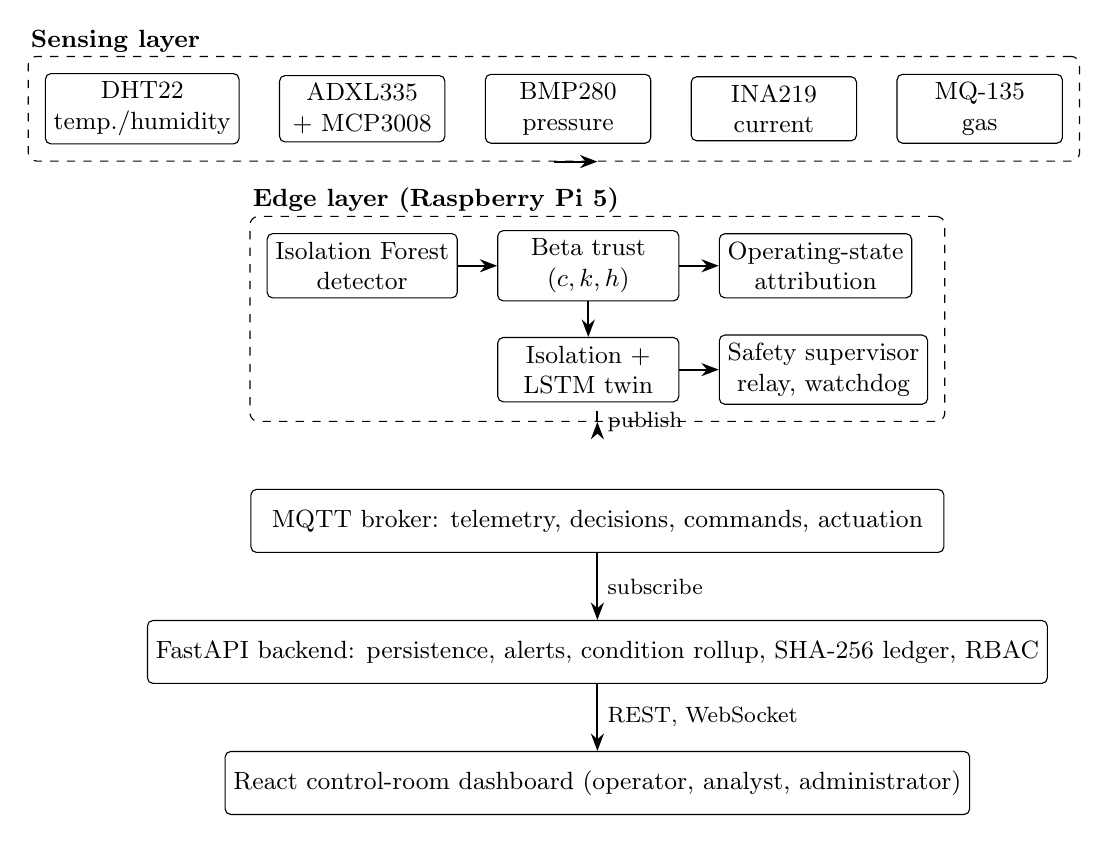
\begin{tikzpicture}[
  box/.style={draw, rounded corners=2pt, align=center, font=\small, minimum height=0.8cm, inner sep=3pt, fill=white},
  fl/.style={-{Stealth[length=2.2mm]}, thick},
  node distance=0.45cm and 0.5cm]
  \node[box, minimum width=2.1cm] (t) {DHT22\\temp./humidity};
  \node[box, minimum width=2.1cm, right=of t] (v) {ADXL335\\+ MCP3008};
  \node[box, minimum width=2.1cm, right=of v] (p) {BMP280\\pressure};
  \node[box, minimum width=2.1cm, right=of p] (c) {INA219\\current};
  \node[box, minimum width=2.1cm, right=of c] (g) {MQ-135\\gas};
  \node[draw, dashed, rounded corners=3pt, fit=(t)(g), inner sep=6pt] (sens) {};
  \node[font=\small\bfseries, anchor=south west, inner sep=1pt] at (sens.north west) {Sensing layer};
  \node[box, below=1.15cm of v, minimum width=2.3cm] (d) {Isolation Forest\\detector};
  \node[box, right=of d, minimum width=2.3cm] (tr) {Beta trust\\($c,k,h$)};
  \node[box, right=of tr, minimum width=2.3cm] (a) {Operating-state\\attribution};
  \node[box, below=0.45cm of tr, minimum width=2.3cm] (h) {Isolation +\\LSTM twin};
  \node[box, right=of h, minimum width=2.3cm] (sv) {Safety supervisor\\relay, watchdog};
  \node[draw, dashed, rounded corners=3pt, fit=(d)(a)(h)(sv), inner sep=6pt] (edge) {};
  \node[font=\small\bfseries, anchor=south west, inner sep=1pt] at (edge.north west) {Edge layer (Raspberry Pi 5)};
  \node[box, below=0.85cm of edge, minimum width=8.8cm] (mq) {MQTT broker: telemetry, decisions, commands, actuation};
  \node[box, below=0.85cm of mq, minimum width=8.8cm] (be) {FastAPI backend: persistence, alerts, condition rollup, SHA-256 ledger, RBAC};
  \node[box, below=0.85cm of be, minimum width=8.8cm] (ui) {React control-room dashboard (operator, analyst, administrator)};
  \draw[fl] (sens.south) -- (edge.north |- sens.south);
  \draw[fl] (d) -- (tr); \draw[fl] (tr) -- (a); \draw[fl] (tr) -- (h); \draw[fl] (h) -- (sv);
  \draw[fl] (edge.south) -- node[right, font=\footnotesize]{publish} (mq.north |- edge.south);
  \draw[fl] (mq) -- node[right, font=\footnotesize]{subscribe} (be);
  \draw[fl] (be) -- node[right, font=\footnotesize]{REST, WebSocket} (ui);
\end{tikzpicture}
\caption{Layered architecture of SHTAPM. All decisions are made on the edge node; the backend observes, persists and audits.}
\label{fig:arch}
\end{figure}

\subsection{Acquisition and Preprocessing}

A sampler reads every driver once per second. A driver that fails does not stop the frame: its last good value is held, and the channel is reported dead only after 5~s of continuous failure, so that brief dropouts of the humidity--temperature sensor when the motor starts are absorbed. Two driver-level safeguards were added after faults observed on the bench: a reader that has failed for 10~s re-opens its device, and an accelerometer axis reading at either rail of the 10-bit converter is treated as a failed read, because it indicates a loose connection rather than a real acceleration.

Raw converter counts are converted to engineering units. With the converter reference $V_{\mathrm{ref}} = 3.3$~V and the accelerometer sensitivity $S = 0.330$~V/$g$, one count corresponds to $\Delta a = V_{\mathrm{ref}} / (1024\, S) \approx 9.77 \times 10^{-3}~g$, and vibration is reported as the deviation from an at-rest baseline captured on the first successful read,
\begin{equation}
v = \Delta a \sqrt{(n_x - n_x^0)^2 + (n_y - n_y^0)^2 + (n_z - n_z^0)^2},
\end{equation}
which is zero for a still motor in any mounting orientation. Motor current is read by a high-side current monitor over a 0.1~$\Omega$ shunt with resolution $I_{\mathrm{LSB}} = 5/32767 \approx 1.526 \times 10^{-4}$~A. The last $W = 30$ samples of each channel form a window, which is processed by an optional median filter, a first-order low-pass filter $y_t = a\,x_t + (1-a)\,y_{t-1}$ and a per-window min--max normalisation $\tilde{x}_i = (x_i - \min_j x_j)/(\max_j x_j - \min_j x_j)$ (a flat window maps to zeros). The deployed configuration uses identity filters ($m = 1$, $a = 1$), and the detector is calibrated on windows prepared identically.

\subsection{Anomaly Detection}

Each $30 \times 6$ window is flattened into a 180-dimensional observation and scored by an Isolation Forest \cite{liu2008iforest}, an ensemble of 100 random binary trees. With $h(\mathbf{x})$ the path length of $\mathbf{x}$ in one tree, the anomaly score is
\begin{equation}
s(\mathbf{x}, \psi) = 2^{-\mathbb{E}[h(\mathbf{x})]/c(\psi)}, \qquad c(\psi) = 2H(\psi-1) - \frac{2(\psi-1)}{\psi},
\end{equation}
where $\psi$ is the sub-sample size, $H(i) \approx \ln i + 0.5772$ and $c(\psi)$ is the average path length of an unsuccessful binary-search-tree lookup. Raw scores are not thresholded directly. The scores of the clean training windows are stored, and the \emph{severity} of a new window is the empirical cumulative distribution value of its score within them,
\begin{equation}
\mathrm{sev}(\mathbf{x}) = \frac{\left|\{ j : s_j^{\mathrm{clean}} \leq s(\mathbf{x}) \}\right|}{N_{\mathrm{clean}}} \in [0,1],
\end{equation}
so that no threshold constant is tied to the model's internal score scale. A window is flagged when $\mathrm{sev} \geq 0.90$. By construction about 10\% of clean windows are flagged: the detector is deliberately a sensitive first stage, and trust and attribution decide which flags matter. The flag is localised to channels by comparing each channel's window variance with that channel's own clean distribution; a channel is flagged when its variance lies in the lowest or highest 10\% of that distribution. The two-sided test catches both spikes and constant spoofs (abnormally low normalised variance) and noisy behaviour (abnormally high variance).

\subsection{Operating-State Attribution}
\label{sec:attribution}

A pump motor is either running or idle, and both its supply current and its vibration reflect that state. Each of the two sensors is therefore an independent witness of the motor state. The rule classifies each channel from the \emph{median} of its raw window, so that impulsive events such as a tap or a one-sample glitch cannot flip the state:
\begin{equation}
s(\mathbf{x}) =
\begin{cases}
\textsc{idle}, & \operatorname{med}(\mathbf{x}) \leq b_{\mathrm{idle}}, \\
\textsc{running}, & \operatorname{med}(\mathbf{x}) \geq b_{\mathrm{run}}, \\
\textsc{unclear}, & \text{otherwise.}
\end{cases}
\end{equation}
For current, $b_{\mathrm{idle}} = 0.05$~A and $b_{\mathrm{run}} = 0.3$~A. Vibration depends on how the sensor is mounted, so its bands are learned from the steady windows of the clean baseline: $b_{\mathrm{idle}}$ is 1.5 times the 99.9th percentile of the idle window medians, and $b_{\mathrm{run}}$ lies midway between $b_{\mathrm{idle}}$ and the 5th percentile of the running window medians, which gives 0.142~$g$ and 0.314~$g$ on the deployed baseline. The gap between the bands is a hysteresis region in which no verdict is given, so motor transitions never produce a violation.

When one channel reports \textsc{idle} and the other \textsc{running}, the machine described by the data is physically impossible and one reading must be false. The suspect is the channel whose state changed most recently while the other stayed constant: a motor that really starts or stops moves both channels together, whereas a single falsified channel moves alone. Algorithm~\ref{alg:attr} summarises the rule. An anomaly is attributed as an \emph{attack} on the suspect when physics is violated and as a \emph{fault} otherwise, and when labels compete the priority is attack, then fault, then none. The rule covers the physically coupled pair of channels; the other channels have no physical partner on the bench and can only be attributed as faults.

\begin{algorithm}[H]
\caption{Operating-state attribution for one window}
\label{alg:attr}
\begin{algorithmic}[1]
\Require raw windows $\mathbf{x}_I$ (current), $\mathbf{x}_V$ (vibration); channel flags $F$; previous states $s_I^{-}, s_V^{-}$
\Ensure attribution label and suspect channel
\State $s_I \gets s(\mathbf{x}_I)$, \; $s_V \gets s(\mathbf{x}_V)$
\If{$\{s_I, s_V\} = \{\textsc{idle}, \textsc{running}\}$}
  \If{$s_I \neq s_I^{-}$ \textbf{and} $s_V = s_V^{-}$} \State suspect $\gets$ current
  \ElsIf{$s_V \neq s_V^{-}$ \textbf{and} $s_I = s_I^{-}$} \State suspect $\gets$ vibration
  \Else \State suspect $\gets$ both
  \EndIf
  \State \Return (\textsc{attack}, suspect, ``physics violation'')
\ElsIf{any channel in $F$ is flagged}
  \State \Return (\textsc{fault}, flagged channels, ``physically consistent anomaly'')
\Else
  \State \Return (\textsc{none}, --, --)
\EndIf
\end{algorithmic}
\end{algorithm}

\subsection{Evidence-Fusing Beta Trust}
\label{sec:trust}

Every channel carries a Beta-reputation state \cite{josang2002beta} $(\alpha, \beta)$ with $\alpha_0 = \beta_0 = 1$ and trust $T = \alpha/(\alpha+\beta) \in [0,1]$. Each window supplies an evidence value $g \in [0,1]$ built from three independent terms.

\paragraph{Consistency $c$.} With the channel's baseline mean $\mu$ and deviation $\sigma$, $z_i = (x_i - \mu)/\sigma$, $r = \sqrt{\tfrac{1}{W}\sum_i z_i^2}$ and $c = 1 - F_r(r)$, where $F_r$ is the empirical distribution of $r$ over the clean windows. A window that resembles typical clean data scores about 0.5; an extreme window scores near 0.

\paragraph{Physical correlation $k$.} $k = 1$ unless the attribution rule finds current and vibration describing an impossible state, in which case the suspect receives $k = 0$ (both channels when the rule cannot tell which one moved). Channels without a physical partner always receive $k = 1$.

\paragraph{Historical reliability $h$.} An exponentially weighted record of past outcomes,
\begin{equation}
h_t = \gamma\, h_{t-1} + (1-\gamma)\, o_t, \qquad \gamma = 0.95,\; h_0 = 1,
\end{equation}
where $o_t = 1$ when the channel was not flagged in window $t$ and $0$ otherwise (half-life of about 13 windows).

The evidence and the update are
\begin{align}
g &= 0.4\,c + 0.3\,k + 0.3\,h, \label{eq:g}\\
\alpha_t &= \lambda\,\alpha_{t-1} + g, \qquad \beta_t = \lambda\,\beta_{t-1} + (1 - g), \qquad \lambda = 0.7. \label{eq:upd}
\end{align}
The forgetting factor gives the trust an effective memory of $1/(1-\lambda) \approx 3.3$ windows. \textbf{Property (steady state).} Under constant evidence $g$, the recursion converges to $\alpha^{*} = g/(1-\lambda)$ and $\beta^{*} = (1-g)/(1-\lambda)$, because $\alpha^{*} = \lambda\alpha^{*} + g$ has the unique fixed point $g/(1-\lambda)$ and likewise for $\beta$, and $\lambda < 1$ makes the map a contraction. Hence
\begin{equation}
T^{*} = \frac{\alpha^{*}}{\alpha^{*} + \beta^{*}} = \frac{g/(1-\lambda)}{g/(1-\lambda) + (1-g)/(1-\lambda)} = g,
\end{equation}
so the trust score settles exactly at the level of the evidence: it is bounded, interpretable and free of drift. Channels are classified as \textbf{Trusted} ($T \geq 0.7$), \textbf{Suspicious} ($0.4 \leq T < 0.7$) or \textbf{Malicious} ($T < 0.4$).

Fig.~\ref{fig:trust} shows the dynamics for an idealised profile: typical clean evidence ($c = 0.5$, $k = 1$), 45 windows of fully adverse evidence ($c = 0$, $k = 0$, flagged), then clean evidence again. Trust falls from Trusted to Malicious within three windows, yet returns to Trusted only 21 windows after the evidence recovers, because $h$ recovers slowly. This asymmetry is intentional: a sensor that has lied must earn its trust back.

\begin{figure}[H]
\centering
\begin{tikzpicture}
\begin{axis}[
  width=0.88\textwidth, height=6cm,
  xlabel={Window index}, ylabel={Value},
  xmin=0, xmax=120, ymin=0, ymax=1.02, ytick={0,0.2,0.4,0.7,1},
  tick label style={font=\footnotesize}, label style={font=\small},
  legend style={at={(0.98,0.04)}, anchor=south east, font=\footnotesize, draw=none, fill=white},
  grid=major, grid style={gray!20}]
\fill[gray!12] (axis cs:30,0) rectangle (axis cs:75,1.02);
\node[font=\footnotesize, anchor=north] at (axis cs:52,1.0) {adverse evidence};
\addplot[thick, black] table[x=t, y=trust] {data/trust.dat};
\addplot[thick, dashed, gray] table[x=t, y=evidence] {data/trust.dat};
\addplot[thin, densely dotted, black, domain=0:120] {0.7};
\addplot[thin, densely dotted, black, domain=0:120] {0.4};
\legend{trust $T$, evidence $g$}
\end{axis}
\end{tikzpicture}
\caption{Response of the trust update (Eqs.~\ref{eq:g}--\ref{eq:upd}) to an idealised evidence profile. Dotted lines mark the 0.7 and 0.4 band limits.}
\label{fig:trust}
\end{figure}

\subsection{Isolation and Bounded Digital-Twin Substitution}
\label{sec:twin}

A channel enters isolation when $T < 0.4$ and is released when $T \geq 0.7$; the Suspicious band in between prevents oscillation. While isolated, its reading is removed from fusion and replaced by a digital-twin reconstruction, and the dashboard marks the value as \textsc{virtual}. The twin is a single-layer unidirectional LSTM \cite{hochreiter1997lstm}. For each time step $t$ of the 30-sample window its input $\mathbf{u}_t$ concatenates the six channel values, with the isolated channel set to zero, and a six-element one-hot mask naming the missing channel:
\begin{align}
\mathbf{i}_t &= \sigma(\mathbf{W}_i \mathbf{u}_t + \mathbf{U}_i \mathbf{h}_{t-1} + \mathbf{b}_i), &
\mathbf{f}_t &= \sigma(\mathbf{W}_f \mathbf{u}_t + \mathbf{U}_f \mathbf{h}_{t-1} + \mathbf{b}_f), \nonumber\\
\mathbf{o}_t &= \sigma(\mathbf{W}_o \mathbf{u}_t + \mathbf{U}_o \mathbf{h}_{t-1} + \mathbf{b}_o), &
\tilde{\mathbf{c}}_t &= \tanh(\mathbf{W}_c \mathbf{u}_t + \mathbf{U}_c \mathbf{h}_{t-1} + \mathbf{b}_c), \nonumber\\
\mathbf{c}_t &= \mathbf{f}_t \odot \mathbf{c}_{t-1} + \mathbf{i}_t \odot \tilde{\mathbf{c}}_t, &
\mathbf{h}_t &= \mathbf{o}_t \odot \tanh(\mathbf{c}_t),
\end{align}
and the reconstruction is $\hat{y} = \mathbf{w}^{\top}\mathbf{h}_{30} + b$. Inputs and target use a fixed z-score scale computed on the clean training data, so that the output converts exactly to engineering units, and the trained weights, the scale and the clean residual statistics are saved as one bundle so that a model can never be loaded with a scale it was not trained on.

The deployed twin reconstructs motor current from vibration. It has 32 hidden units and was trained with the Adam optimiser (learning rate 0.01, 30 epochs, mean-squared-error loss) on three bench recordings, holding out the last 15\% of each; no training window spans two recordings or a time gap. The ambient channels are excluded from its input, because a leave-one-recording-out study (Section~\ref{sec:ablation}) showed that they carry no information about current and shift from day to day.

Substitution is bounded. An uncertainty value $u = \min(t_s/60, 1)$ grows with the elapsed substitution time $t_s$ in seconds; when $u$ exceeds the cap of 0.8 (after 48~s) the self-healing layer signals that the budget is nearly spent, and after 60~s of continuous substitution it escalates to a safe stop. A second escalation path compares the live reading with the twin and escalates when their divergence exceeds a threshold; it is implemented and tested but disabled in the deployed configuration, because on clean held-out data a $3\sigma$ threshold would have produced false escalations in 4.5\% of windows, which is not acceptable for an action that stops the plant.

\subsection{Safety Supervisor}

The supervisor is the only component allowed to switch the pump relay. It acts on four causes: an operator command, a self-healing escalation, a dry-run signature (pump commanded on, past a 5~s spin-up grace, with the current inside the dry-run band for three consecutive frames), and a watchdog that fires when no healthy frame has arrived for 10~s while the pump runs. Every autonomous stop \emph{latches}: the pump stays off until an administrator restarts it through a confirmation. The relay is forced off at start-up and at shutdown, and the service manager releases the relay pin after a crash, so every failure mode ends with the pump stopped. Relay commands travel on their own MQTT topic, separate from scenario injections, so an injected test scenario can never reach the relay (Fig.~\ref{fig:safety}).

\begin{figure}[H]
\centering
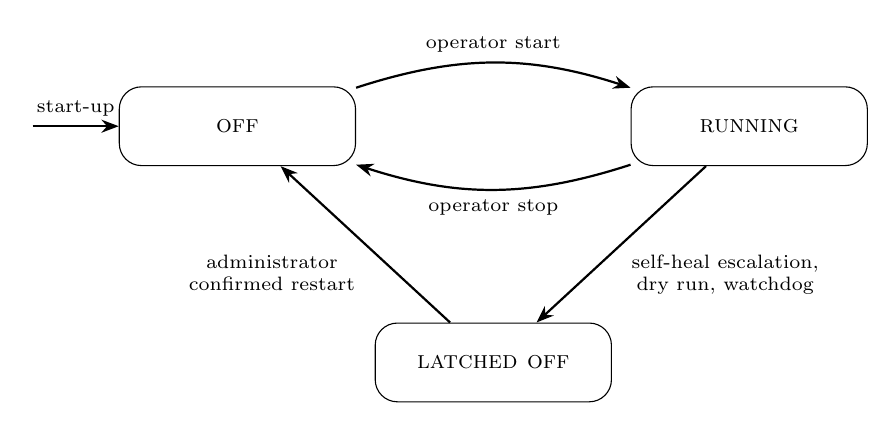
\begin{tikzpicture}[
  st/.style={draw, rounded corners=8pt, minimum width=3.0cm, minimum height=1.0cm, align=center, font=\small, fill=white},
  tr/.style={-{Stealth[length=2.2mm]}, thick},
  tl/.style={font=\scriptsize, align=center}]
  \node[st] (off) at (0,0) {\textsc{off}};
  \node[st] (run) at (6.5,0) {\textsc{running}};
  \node[st] (lat) at (3.25,-3.0) {\textsc{latched off}};
  \draw[tr] (off) to[bend left=18] node[tl, above]{operator start} (run);
  \draw[tr] (run) to[bend left=18] node[tl, below]{operator stop} (off);
  \draw[tr] (run) -- node[tl, below right]{self-heal escalation,\\dry run, watchdog} (lat);
  \draw[tr] (lat) -- node[tl, below left]{administrator\\confirmed restart} (off);
  \draw[tr] (-2.6,0) -- node[tl, above]{start-up} (off);
\end{tikzpicture}
\caption{State machine of the safety supervisor.}
\label{fig:safety}
\end{figure}

\subsection{Tamper-Evident Decision Ledger}

Safety-relevant events are appended to a hash chain \cite{haber1991timestamp}. For block $n$ with timestamp $\tau_n$ and payload $P_n$,
\begin{align}
\mathrm{ph}_n &= \mathrm{SHA256}\big(\mathrm{canon}(P_n)\big), \\
H_n &= \mathrm{SHA256}\big(n \,\|\, \tau_n \,\|\, \mathrm{ph}_n \,\|\, H_{n-1}\big), \qquad H_{-1} = 0^{64},
\end{align}
where $\mathrm{canon}$ serialises the payload as JSON with sorted keys and no insignificant whitespace, so that equal payloads always give equal digests. Modifying any field of block $n$ changes $\mathrm{ph}_n$ or $H_n$ and breaks the link stored in block $n+1$. A verifier recomputes the three digests of every block in order and reports the index of the first block that does not match.

\subsection{Complete Pipeline Execution}

Algorithm~\ref{alg:pipeline} gives one decision cycle of the complete framework.

\begin{algorithm}[H]
\caption{One decision cycle on the edge node}
\label{alg:pipeline}
\begin{algorithmic}[1]
\Require new frame $\mathbf{y}_t$; trust states; isolation set $\mathcal{I}$; substitution clocks
\Ensure published decision, served values, relay state
\State append $\mathbf{y}_t$ to the window; \textbf{if} fewer than $W$ frames \textbf{then return}
\State compute $\mathrm{sev}$ and channel flags $F$ (Section 4.3)
\State attribute with Algorithm~\ref{alg:attr}; set $k$ for the suspect channel
\For{each channel $i$}
  \State compute $c_i$, update $h_i$, form $g_i$, update $(\alpha_i, \beta_i)$ by Eq.~\eqref{eq:upd}
  \If{$T_i < 0.4$} \State add $i$ to $\mathcal{I}$ \ElsIf{$T_i \geq 0.7$ \textbf{and} $i \in \mathcal{I}$} \State release $i$; reset its clock \EndIf
\EndFor
\For{each $i \in \mathcal{I}$}
  \State serve $\hat{y}_i \gets$ twin reconstruction; advance clock $t_s$
  \If{$t_s \geq 60$~s} \State request latched safe stop \EndIf
\EndFor
\State supervisor checks watchdog and dry-run; switches relay if required
\State publish decision, telemetry and actuation; backend chains ledger events on transitions
\end{algorithmic}
\end{algorithm}

%==============================================================
\section{Prototype, Data and Evaluation Protocol}
\label{sec:setup}

\subsection{Prototype Rig}

A 130-size brushed DC motor, powered from a 5~V supply, stands in for the pump. A Raspberry~Pi~5 is the edge node. Table~\ref{tab:rig} lists the sensing layer and the configuration used in the experiments. Motor current is measured by the current monitor in series with the motor supply, and vibration by the accelerometer taped to the motor body. The gas channel and the pump relay are implemented end to end in software (a gas-sensor driver with its voltage-divider signal conditioning, and a supervised relay with latching stops); in the reported experiments both were driven through configurable emulated sources that share the data path with the physical drivers. They therefore carry no weight in any result of this paper, and the evaluation of attribution, trust and self-healing rests on the physical current, vibration, temperature, humidity and pressure channels.

\begin{table}[H]
\centering
\caption{Sensing layer and prototype configuration}
\label{tab:rig}
\small
\begin{tabularx}{\textwidth}{@{}P{2.4cm} P{3.6cm} P{3.0cm} X@{}}
\toprule
\textbf{Channel} & \textbf{Device} & \textbf{Interface} & \textbf{Prototype configuration} \\
\midrule
Temperature, humidity & DHT22 & GPIO17 & Physical sensor \\
Vibration & ADXL335 via MCP3008 (10-bit) & SPI0, channels 0--2 & Physical sensor on the motor body \\
Pressure & BMP280 & I\textsuperscript{2}C 0x76 & Physical sensor \\
Motor current & INA219, 0.1~$\Omega$ shunt & I\textsuperscript{2}C 0x40 & Physical sensor in series with the supply \\
Gas & MQ-135 & MCP3008 channel 3 & Driver implemented; emulated source in experiments \\
Pump relay & Relay module, normally open & GPIO27 & Supervisor implemented; in-memory relay in experiments \\
\bottomrule
\end{tabularx}
\end{table}

\subsection{Datasets and Recordings}

\textbf{Main dataset.} A 51.4-minute recording of clean operation with all physical sensors in place: 2,609 frames, no frame gap longer than 2~s, and 21 motor runs switched by hand at random intervals (motor on 47\% of the time). It is used to fit the baseline and for the injection experiments. Fig.~\ref{fig:baseline} shows current and vibration over the recording; the motor runs are clearly visible in both channels, with switch-on current surges and occasional vibration spikes from handling the rig. A first 70-minute recording was rejected by a recording check because the accelerometer had shifted on the first motor run, which made idle and running vibration indistinguishable; the check is now run within minutes of starting any recording.

\begin{figure}[H]
\centering
\begin{tikzpicture}
\begin{groupplot}[
  group style={group size=1 by 2, vertical sep=0.45cm, xlabels at=edge bottom, xticklabels at=edge bottom},
  width=0.94\textwidth, height=4.4cm, xmin=0, xmax=51.5,
  xlabel={Time (min)}, tick label style={font=\footnotesize}, label style={font=\small},
  grid=major, grid style={gray!20}, restrict y to domain=-1:2, clip=true]
\nextgroupplot[ylabel={Current (A)}, ymin=-0.05, ymax=1.2]
\addplot[black, thin] table[x=t, y=current] {data/baseline_series.dat};
\nextgroupplot[ylabel={Vibration ($g$)}, ymin=-0.05, ymax=1.5]
\addplot[black, thin] table[x=t, y=vibration] {data/baseline_series.dat};
\end{groupplot}
\end{tikzpicture}
\caption{Motor current and vibration over the 51.4-minute baseline recording (every third sample shown; clipped above 1.2~A and 1.5~$g$).}
\label{fig:baseline}
\end{figure}

\textbf{Earlier recordings.} A 7.2-hour idle recording, a 19-minute on/off cycling recording and a 25-minute motor-running recording of the same rig are used to test robustness across motor states and days, and a 70-minute cycling recording is used for the twin study.

\textbf{Public dataset.} SWaT.A1 \cite{goh2016swat} is used for detection: the detectors are fitted on its normal-operation file only and evaluated on its attack file (14,997 windows, 35 attack events).

Fig.~\ref{fig:medians} plots the median current against the median vibration of each 30-sample window of the main recording together with the state bands. The windows form two well-separated clusters, only 3 of 258 windows fall in the transition region, and the two off-diagonal regions contain no windows. These regions are the physically impossible states that the attribution rule treats as evidence of falsification.

\begin{figure}[H]
\centering
\begin{tikzpicture}
\begin{axis}[
  width=0.8\textwidth, height=7cm,
  xlabel={Window median current (A)}, ylabel={Window median vibration ($g$)},
  xmin=-0.05, xmax=1.0, ymin=-0.05, ymax=1.1,
  tick label style={font=\footnotesize}, label style={font=\small},
  legend style={at={(0.02,0.98)}, anchor=north west, font=\footnotesize, draw=none, fill=white, fill opacity=0.9, text opacity=1},
  scatter/classes={idle={mark=o, black}, running={mark=triangle, black}, transition={mark=square*, gray}}]
\fill[gray!12] (axis cs:0.3,-0.05) rectangle (axis cs:1.0,0.142);
\fill[gray!12] (axis cs:-0.05,0.314) rectangle (axis cs:0.05,1.1);
\node[font=\scriptsize, align=center] at (axis cs:0.65,0.06) {impossible: current running,\\vibration idle};
\node[font=\scriptsize, align=center, rotate=90] at (axis cs:0.0,0.7) {impossible};
\addplot[scatter, only marks, mark size=1.6pt, scatter src=explicit symbolic] table[x=current, y=vibration, meta=state] {data/window_medians.dat};
\draw[densely dashed] (axis cs:0.05,-0.05) -- (axis cs:0.05,1.1);
\draw[densely dashed] (axis cs:0.3,-0.05) -- (axis cs:0.3,1.1);
\draw[densely dotted] (axis cs:-0.05,0.142) -- (axis cs:1.0,0.142);
\draw[densely dotted] (axis cs:-0.05,0.314) -- (axis cs:1.0,0.314);
\legend{idle windows, running windows, transition windows}
\end{axis}
\end{tikzpicture}
\caption{Window medians of the baseline recording with the motor-state bands (dashed: current bands 0.05~A and 0.3~A; dotted: learned vibration bands 0.142~$g$ and 0.314~$g$; shaded: physically impossible states).}
\label{fig:medians}
\end{figure}

\subsection{Injection Protocol}

Ground truth on real hardware is obtained by injecting the eight fault and attack types of Table~\ref{tab:inject} into the recordings at random onsets and replaying the result through the exact live composition of the edge pipeline; ten episodes are injected per scenario. In the live path the injection is applied inside the edge, after acquisition and before detection, so it takes the same path that a real falsified reading would take. Attacks are further grouped \emph{by measurement}: those whose injected reading crosses into the opposite motor state (physically impossible) and those that stay within the true state. Injection magnitudes are fixed evaluation settings, and no threshold was tuned on evaluation data.

\begin{table}[H]
\centering
\caption{Fault and attack injections ($x_t$: true reading, $t$: samples since onset)}
\label{tab:inject}
\small
\begin{tabular}{@{}l l l@{}}
\toprule
\textbf{Injection} & \textbf{Class} & \textbf{Injected value} \\
\midrule
Gradual drift & Fault & $x_t + r\,t$ \\
Sudden spike & Fault & $x_t + A$ on the active samples \\
Stuck sensor & Fault & value frozen at onset \\
Bias injection & Attack & $x_t + b$ \\
Ramp injection & Attack & $x_t + r\,t$ \\
Replay & Attack & the channel's own earlier recording \\
Constant spoof & Attack & a constant value $v$ \\
Adaptive stealth & Attack & $x_t + \mathrm{clip}(r\,t, -\delta, \delta)$, kept below a residual bound $\delta$ \\
\bottomrule
\end{tabular}
\end{table}

\subsection{Evaluation Metrics}

Detection is scored by precision, recall, $F_1$ and false-positive rate over windows, and, because window-level scores favour long attacks, by \emph{event coverage} (the number of distinct attack events flagged at least once). Attribution is scored for each injected episode on the injected channel in two ways: \emph{settled} (the majority label over the episode's flagged windows) and \emph{episode} (attack if any flagged window was attributed attack). Faults are scored the same way, so a false accusation counts against the method. The \emph{false-attack rate} is the fraction of channel-windows of clean data attributed attack. A rule that labels everything ``attack'' would score perfectly on attacks, so the summary metric is the balanced accuracy
\begin{equation}
\mathrm{BA} = \tfrac{1}{2}\left(\mathrm{Recall}_{\mathrm{attack}} + \mathrm{Recall}_{\mathrm{fault}}\right).
\end{equation}
Self-healing is scored by the time to isolate, the share of the attack served by the twin, the median error of the served value against the true reading and the time to release; the twin's accuracy is also reported as skill against a predictor that always outputs the training mean, $\mathrm{skill} = 1 - \mathrm{RMSE}_{\mathrm{twin}}/\mathrm{RMSE}_{\mathrm{mean}}$.

\subsection{Implementation Environment}

\begin{table}[H]
\centering
\caption{Software and deployed parameters}
\label{tab:params}
\small
\begin{tabularx}{\textwidth}{@{}P{3.5cm} X@{}}
\toprule
\textbf{Item} & \textbf{Configuration} \\
\midrule
Edge node & Raspberry~Pi~5, Raspberry~Pi~OS 64-bit, Python $\geq$ 3.11, systemd service \\
Messaging & Eclipse Mosquitto 2.0 on the Pi; paho-mqtt 1.6 \\
Backend & FastAPI 0.110, SQLAlchemy 2.0 (SQLite in the bench setup; PostgreSQL with TimescaleDB as the deployment target), JSON Web Tokens (15-minute access, 7-day rotating refresh) \\
Dashboard & React 18.2, TypeScript 5.4, Vite 5.2 \\
Detector & scikit-learn 1.5 Isolation Forest, 100 trees, window 30, flag at severity 0.90 \\
Trust & weights 0.4/0.3/0.3, $\lambda = 0.7$, $\gamma = 0.95$, bands 0.7 and 0.4 \\
Twin & PyTorch 2.2, 1-layer LSTM, 32 hidden units, Adam 0.01, 30 epochs \\
Supervisor & substitution budget 60~s, uncertainty cap 0.8, watchdog 10~s, dry-run grace 5~s and 3 frames \\
Testing & pytest 8 and Vitest 1.6: 2,358 Python and 259 dashboard tests passed, none failed \\
\bottomrule
\end{tabularx}
\end{table}

%==============================================================
\section{Experimental Results and Discussion}
\label{sec:results}

\subsection{False Alarms on Clean Data}

The baseline was fitted on the first 80\% of the main recording and scored on the remaining 493 windows, all of them clean, so that every alarm is a false alarm (Table~\ref{tab:holdout}). The detector flagged about one window in five, as intended for a sensitive first stage, yet no channel ever entered the Malicious band and none was isolated, because trust and the physics rule filter the flags. The median clean trust of every channel lies above 0.7, which guarantees that an isolated channel can always be released once its input is clean.

\begin{table}[H]
\centering
\caption{Hold-out check of the deployed baseline on clean data}
\label{tab:holdout}
\small
\begin{tabularx}{\textwidth}{@{}X l@{}}
\toprule
\textbf{Measure} & \textbf{Result} \\
\midrule
Windows flagged by the Isolation Forest (threshold 0.90) & 98 of 493 (19.9\%) \\
Channel-windows with trust in the Malicious band & 0 on every channel \\
Channels isolated at the end of the hold-out & None \\
Median clean trust per channel & 0.75--0.83 (all $\geq$ 0.7) \\
Learned vibration bands & idle $\leq$ 0.142~$g$, running $\geq$ 0.314~$g$ \\
Steady idle windows classified idle & 152 of 152 (100\%) \\
\bottomrule
\end{tabularx}
\end{table}

\subsection{Detection on Bench Data}

On the main recording, the deployed detector flagged every injected fault (60 of 60) and every injected attack (120 of 120) at a nominal 5\% clean-flag threshold, with a median delay of 6 samples. Window flags alone are not alarms; they become alarms only through trust and attribution.

\subsection{Fault and Attack Attribution}

Table~\ref{tab:attr} reports attribution of the deployed rule per scenario. State-crossing bias injection was attributed correctly in all ten detected episodes and replay of the other motor state in nine of ten; spikes and stuck sensors were always kept as faults. Grouped by physical measurement, the rule attributed \textbf{73\%} of state-crossing attacks correctly at episode level (32 of 44; 66\% settled) and kept \textbf{85\%} of faults as faults (23 of 27), with \textbf{zero} false attacks on 2,552 clean channel-windows. Attacks that stay within the true motor state were never attributed as attacks (0 of 23): such readings are physically consistent, which is the limit analysed in Section~\ref{sec:ablation}. Most of the remaining fault errors are drifts, which share their waveform with ramp attacks.

\begin{table}[H]
\centering
\caption{Attribution on the main recording (deployed rule, 10 injections per scenario)}
\label{tab:attr}
\small
\begin{tabularx}{\textwidth}{@{}X l c c@{}}
\toprule
\textbf{Scenario} & \textbf{Truth} & \textbf{Detected} & \textbf{Correctly attributed (settled)} \\
\midrule
Sudden spike (2 samples) & Fault & 8 & 8 \\
Stuck sensor & Fault & 10 & 10 \\
Gradual drift & Fault & 9 & 5 \\
Constant spoof, crossing state & Attack & 10 & 6 \\
Bias injection, crossing state & Attack & 10 & 10 \\
Replay of the other motor state & Attack & 10 & 9 \\
Ramp injection & Attack & 9 & 4 \\
Constant spoof, within state & Attack & 10 & 0 \\
Bias injection, within state & Attack & 9 & 0 \\
Adaptive stealth injection & Attack & 9 & 0 \\
\midrule
Clean data (2,552 channel-windows) & None & -- & \textbf{0 false attacks (0.0\%)} \\
\bottomrule
\end{tabularx}
\end{table}

\subsection{Robustness Across Recordings and Real Physical Events}

The behaviour is stable across motor states and days (Table~\ref{tab:streams}): on a 7.2-hour idle recording all 120 state-crossing attacks were attributed correctly, on a 19-minute cycling recording all 12, and on a 25-minute running recording 63 of 70, with at most 0.1\% false attacks on clean data. To check that real disturbances are not mistaken for attacks, a guided session produced genuine physical events on the rig (Table~\ref{tab:events}). No real event was attributed as an attack, apart from two windows at a motor switch-on, and the only isolation was of an accelerometer that had genuinely lost power.

\begin{table}[H]
\centering
\caption{Attribution of the deployed rule on earlier recordings of the rig}
\label{tab:streams}
\small
\begin{tabularx}{\textwidth}{@{}X c c c@{}}
\toprule
\textbf{Recording} & \textbf{State-crossing attacks} & \textbf{Faults kept as faults} & \textbf{False attacks, clean} \\
\midrule
Idle, 7.2 h & 120/120 (100\%) & 39/79 (49\%)$^{*}$ & 0/4,742 (0.0\%) \\
Cycling, 19 min & 12/12 (100\%) & 5/5 (100\%) & 1/928 (0.1\%) \\
Running, 25 min & 63/70 (90\%) & 36/42 (86\%) & 2/1,594 (0.1\%) \\
\bottomrule
\multicolumn{4}{@{}l}{\footnotesize $^{*}$All idle fault errors are drifts; spikes and stuck sensors were 39/39 correct.}
\end{tabularx}
\end{table}

\begin{table}[H]
\centering
\caption{Attribution of real physical events on the rig}
\label{tab:events}
\small
\begin{tabularx}{\textwidth}{@{}P{6.3cm} P{4.6cm} X@{}}
\toprule
\textbf{Real event} & \textbf{Attribution} & \textbf{Isolation} \\
\midrule
Quiet idle & None or fault & None \\
Motor run, untouched & Two attack windows at switch-on, then fault or none & None \\
Tap on the accelerometer, motor off or running & Fault only & None \\
Accelerometer power removed, motor off & Fault only & None \\
Accelerometer power removed, motor running & Fault only & Vibration (broken sensor) \\
\bottomrule
\end{tabularx}
\end{table}

\subsection{Self-Healing}

Table~\ref{tab:heal} reports self-healing for state-crossing attacks on the current channel. The twin used here was not trained on this recording, so the result is out of sample. The twin removes 79--87\% of the error that the falsified reading would otherwise have introduced (Fig.~\ref{fig:healerr}); on its own held-out data it has a skill of $+47.3\%$ (RMSE 0.188~A against 0.357~A for the mean predictor).

\begin{table}[H]
\centering
\caption{Self-healing on the main recording (12 attacks per scenario)}
\label{tab:heal}
\small
\begin{tabularx}{\textwidth}{@{}X c c@{}}
\toprule
\textbf{Measure} & \textbf{Bias injection} & \textbf{Constant spoof} \\
\midrule
Attacks isolated & 10/12 & 10/12 \\
Time to isolate, median & 17.5 samples ($\approx$ 21~s) & 15 samples ($\approx$ 18~s) \\
Share of attack served by the twin, median & 52\% & 74\% \\
Error without self-healing, median & 0.60~A & 0.57~A \\
Error of the twin's value, median & \textbf{0.079~A} & \textbf{0.12~A} \\
Time to release, median & 38.5 samples & 38.5 samples \\
False isolations on clean data & 0 & 0 \\
\bottomrule
\end{tabularx}
\end{table}

\begin{figure}[H]
\centering
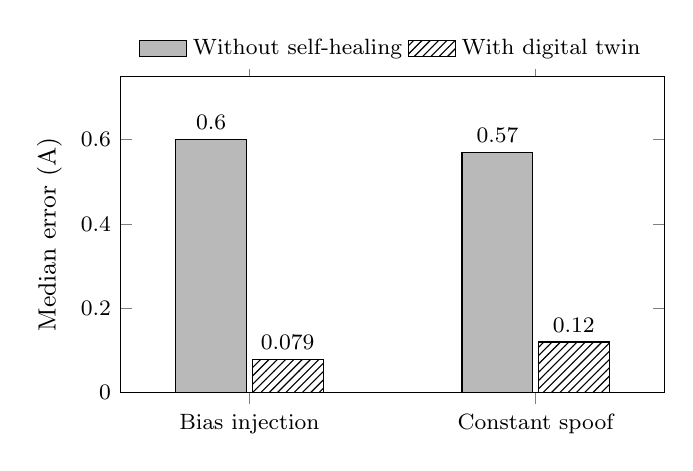
\begin{tikzpicture}
\begin{axis}[
  ybar, area legend, bar width=0.9cm, width=0.7\textwidth, height=5.6cm,
  ylabel={Median error (A)}, ymin=0, ymax=0.75,
  symbolic x coords={Bias injection, Constant spoof}, xtick=data, enlarge x limits=0.45,
  nodes near coords, nodes near coords style={font=\footnotesize, /pgf/number format/fixed, /pgf/number format/precision=3},
  legend style={at={(0.5,1.02)}, anchor=south, legend columns=2, draw=none, font=\footnotesize},
  tick label style={font=\footnotesize}, label style={font=\small}]
\addplot[fill=gray!55, draw=black] coordinates {(Bias injection,0.60) (Constant spoof,0.57)};
\addplot[fill=white, draw=black, postaction={pattern=north east lines}] coordinates {(Bias injection,0.079) (Constant spoof,0.12)};
\legend{Without self-healing, With digital twin}
\end{axis}
\end{tikzpicture}
\caption{Median error of the served current value with and without the digital twin.}
\label{fig:healerr}
\end{figure}

\subsection{Live Evaluation on the Running System}

The scenarios of Table~\ref{tab:hil} were run on the complete system, with the edge on the Raspberry~Pi, the backend and dashboard on a laptop, and the motor under the physical sensors. A constant spoof of the current reading to 0~A while the motor ran was attributed as an attack after 23~s and the channel was isolated and served by the twin; a +0.8~A bias with the motor off was attributed as an attack after 19~s; and a stuck current sensor was reported as a fault.

\begin{table}[H]
\centering
\caption{Hardware-in-the-loop evaluation matrix and status}
\label{tab:hil}
\small
\begin{tabularx}{\textwidth}{@{}l P{5.6cm} P{3.6cm} X@{}}
\toprule
\textbf{ID} & \textbf{Scenario} & \textbf{Expected} & \textbf{Observed} \\
\midrule
HT-01 & Sensor diagnostic on the Pi & All sensors in range & Verified \\
HT-02 & Motor cycled by hand, live dashboard & Six channels at 1~Hz, no attack & Verified \\
HT-03 & Humidity--temperature dropout at motor start & Last value held & Verified \\
HT-04 & Constant spoof to 0~A, motor running, 40~s & Attack, isolation, virtual value & Attack after 23~s; isolated \\
HT-05 & Bias +0.8~A, motor off, 40~s & Attack on current & Attack after 19~s; no false trip \\
HT-06 & Stuck current sensor, motor running & Fault, not attack & Fault \\
HT-07 & Attack held beyond the 60~s budget & Latched safe stop & Pump trip, latched \\
HT-08 & Second isolation after a release & No premature trip & Verified \\
HT-09 & Ledger verification of the session & Chain intact & 200 of 200 blocks \\
HT-10 & Loose converter wire (all channels at the rail) & Readings rejected & Verified \\
HT-11 & Small within-state bias on running current & Not attributable (physical limit) & As expected \\
\bottomrule
\end{tabularx}
\end{table}

A later run of the same constant-spoof scenario, captured for this paper, is traced step by step by its ledger (Fig.~\ref{fig:ui} and Table~\ref{tab:timeline}). The spoof was injected at 12:22:56; at 12:23:17, 21~s later, the current channel's trust fell below 0.4 and the channel was isolated, with the twin serving 0.791~A while the sensor reported 0~A, which is consistent with the running motor. The injection lasted 40~s, but trust recovers only after the window is clean again, so the channel was still isolated when its 60~s budget expired: at 12:24:17, exactly 60~s after isolation, the supervisor performed a latched safe stop, and the channel was released at 12:24:21.

\begin{table}[H]
\centering
\caption{Ledger timeline of one live constant-spoof incident}
\label{tab:timeline}
\small
\begin{tabular}{@{}l l@{}}
\toprule
\textbf{Time} & \textbf{Event} \\
\midrule
12:22:56 & Scenario injected: constant spoof of current to 0~A, 40~s \\
12:23:17 & Trust of current below 0.4; channel isolated; twin serves 0.791~A \\
12:23:17 & Alert raised: attack on current \\
12:24:17 & Isolation reaches 60~s: latched safe stop; alert raised \\
12:24:21 & Current released from isolation \\
-- & Verifier: chain intact over all 200 blocks \\
\bottomrule
\end{tabular}
\end{table}

\begin{figure}[H]
\centering
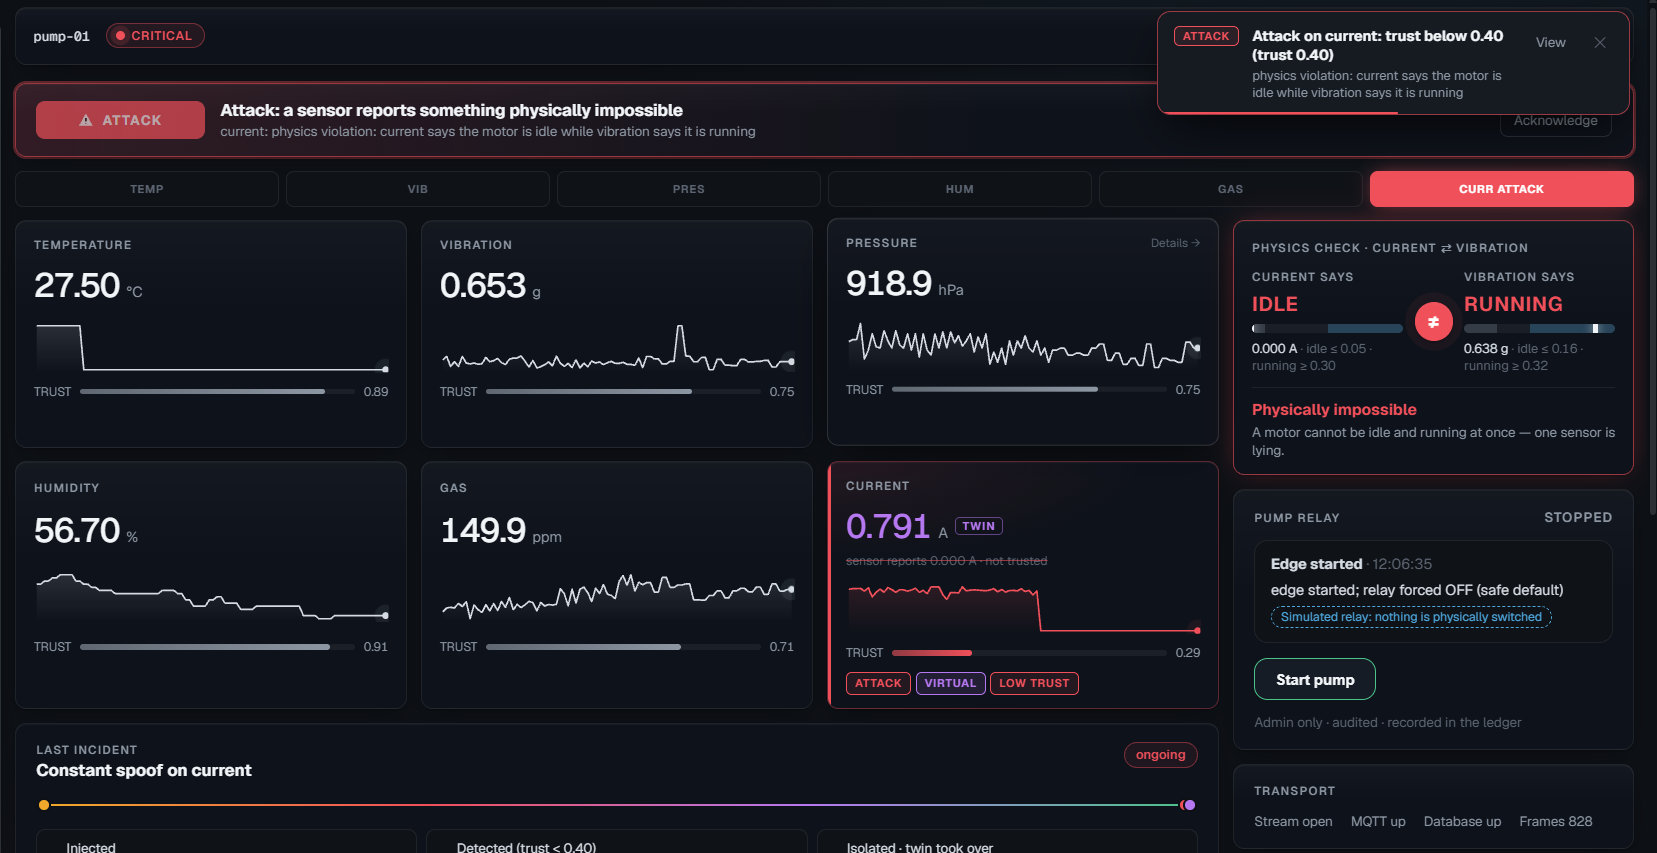
\includegraphics[width=\textwidth]{figures/controlroom-attack.png}
\caption{Control room during the constant-spoof attack: the physics panel reports an impossible state (current idle, vibration running), the channel is attributed as attack and isolated, and the twin's value (0.791~A) is shown in place of the sensor's 0~A.}
\label{fig:ui}
\end{figure}

\subsection{Detection on the SWaT Dataset}

Table~\ref{tab:swat} reports detection on SWaT.A1 with every detector's threshold set to its own nominal 5\% clean-flag rate on the normal-operation data; no attack labels were used to choose thresholds. The two metrics pull apart (Fig.~\ref{fig:swat}): the z-score detector has the best window-level $F_1$ but misses 22 of the 35 attacks, whereas the Isolation Forest flags almost every attack event, trading precision for coverage. In SHTAPM this trade is deliberate, because the trust engine and the physics rule remove the detector's false alarms downstream (Table~\ref{tab:holdout}). The results also identify a direct improvement: low-pass filtering raises the Isolation Forest's $F_1$ from 0.370 to 0.555 at equal event coverage, and the combined detector raises it by 70\% while flagging 33 of 35 events.

\begin{table}[H]
\centering
\caption{Detection on SWaT.A1 at a nominal 5\% clean-flag threshold}
\label{tab:swat}
\small
\begin{tabularx}{\textwidth}{@{}X c c c c c@{}}
\toprule
\textbf{Detector} & \textbf{Precision} & \textbf{Recall} & $\mathbf{F_1}$ & \textbf{FPR} & \textbf{Events (of 35)} \\
\midrule
Isolation Forest, deployed preprocessing & 0.418 & 0.332 & 0.370 & 0.065 & 32 \\
Isolation Forest with low-pass filter & 0.548 & 0.562 & 0.555 & 0.065 & 33 \\
Per-channel z-score & 0.799 & 0.687 & 0.739 & 0.024 & 13 \\
Isolation Forest on standardised windows & 0.766 & 0.651 & 0.704 & 0.028 & 23 \\
Maximum of z-score and low-pass Isolation Forest & 0.543 & 0.746 & 0.629 & 0.089 & 33 \\
\bottomrule
\end{tabularx}
\end{table}

\begin{figure}[H]
\centering
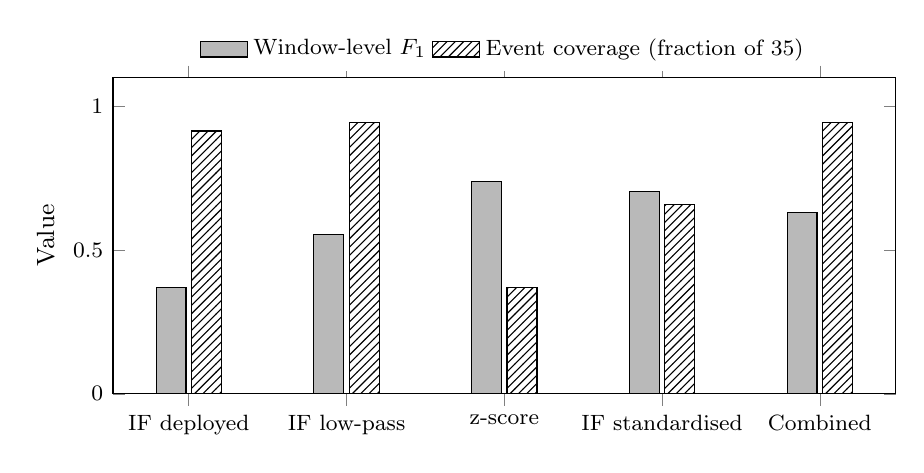
\begin{tikzpicture}
\begin{axis}[
  ybar, area legend, bar width=0.38cm, width=0.95\textwidth, height=5.6cm,
  ymin=0, ymax=1.1, ylabel={Value},
  symbolic x coords={IF deployed, IF low-pass, z-score, IF standardised, Combined},
  xtick=data, x tick label style={font=\footnotesize, align=center}, enlarge x limits=0.12,
  legend style={at={(0.5,1.02)}, anchor=south, legend columns=2, draw=none, font=\footnotesize},
  tick label style={font=\footnotesize}, label style={font=\small}]
\addplot[fill=gray!55, draw=black] coordinates {(IF deployed,0.370) (IF low-pass,0.555) (z-score,0.739) (IF standardised,0.704) (Combined,0.629)};
\addplot[fill=white, draw=black, postaction={pattern=north east lines}] coordinates {(IF deployed,0.914) (IF low-pass,0.943) (z-score,0.371) (IF standardised,0.657) (Combined,0.943)};
\legend{Window-level $F_1$, Event coverage (fraction of 35)}
\end{axis}
\end{tikzpicture}
\caption{Window-level $F_1$ and event coverage on SWaT.A1 (Combined: maximum of z-score and low-pass Isolation Forest).}
\label{fig:swat}
\end{figure}

\subsection{System Performance}

The edge sustained its 1~Hz cycle of acquisition, detection, trust, attribution, self-healing and publication throughout the 51.4-minute session with no frame gap longer than 2~s, so one decision cycle fits within the sampling period. The path from broker to backend to WebSocket client added a 95th-percentile latency of 3--5~ms, so the sensor-to-screen latency is dominated by the 1~s sampling interval and stays within the 2~s requirement.

%==============================================================
\section{Ablation and Robustness Analysis}
\label{sec:ablation}

\subsection{Trend-Sign Rule versus Operating-State Rule}

The first attribution rule implemented in the project compared the up/down trend of current and vibration within each window and labelled an anomaly an attack when the trends disagreed. Table~\ref{tab:ablate} compares it with the operating-state rule on the same injected episodes. The trend-sign rule's high attack recall is not discrimination: it labelled half of the physically consistent attacks and almost two thirds of genuine faults as attacks, and it raised false attacks on clean data. The operating-state rule gives up some recall to remove false accusations entirely and to keep faults as faults, raising balanced accuracy from 60\% to 79\% (Fig.~\ref{fig:attribcompare}). For an operator, an accusation that is never false on clean data is the property that matters.

\begin{table}[H]
\centering
\caption{Attribution rules compared on the main recording}
\label{tab:ablate}
\small
\begin{tabularx}{\textwidth}{@{}X c c@{}}
\toprule
\textbf{Measure} & \textbf{Trend-sign rule} & \textbf{Operating-state rule} \\
\midrule
State-crossing attacks, episode & 35/42 (83\%) & 32/44 (73\%) \\
State-crossing attacks, settled & 4/42 (10\%) & 29/44 (66\%) \\
Within-state attacks, episode & 12/23 (52\%) & 0/23 (0\%) \\
Faults kept as faults, episode & 10/27 (37\%) & 23/27 (85\%) \\
False attacks on clean data & 23/2,552 (0.9\%) & \textbf{0/2,552 (0.0\%)} \\
Balanced accuracy, episode & 60\% & \textbf{79\%} \\
\bottomrule
\end{tabularx}
\end{table}

\begin{figure}[H]
\centering
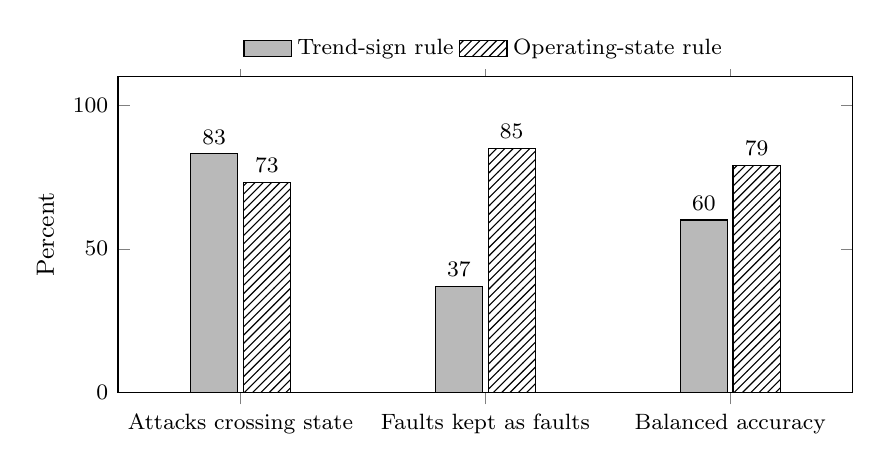
\begin{tikzpicture}
\begin{axis}[
  ybar, area legend, bar width=0.6cm, width=0.9\textwidth, height=5.6cm,
  ymin=0, ymax=110, ylabel={Percent},
  symbolic x coords={Attacks crossing state, Faults kept as faults, Balanced accuracy},
  xtick=data, enlarge x limits=0.25,
  nodes near coords, nodes near coords style={font=\footnotesize, /pgf/number format/fixed, /pgf/number format/precision=0},
  legend style={at={(0.5,1.02)}, anchor=south, legend columns=2, draw=none, font=\footnotesize},
  tick label style={font=\footnotesize}, label style={font=\small}]
\addplot[fill=gray!55, draw=black] coordinates {(Attacks crossing state,83) (Faults kept as faults,37) (Balanced accuracy,60)};
\addplot[fill=white, draw=black, postaction={pattern=north east lines}] coordinates {(Attacks crossing state,73) (Faults kept as faults,85) (Balanced accuracy,79)};
\legend{Trend-sign rule, Operating-state rule}
\end{axis}
\end{tikzpicture}
\caption{Episode-level attribution of the two rules.}
\label{fig:attribcompare}
\end{figure}

\subsection{Twin Input Ablation}

Table~\ref{tab:loco} shows the leave-one-recording-out evaluation that determined the twin's inputs: models were trained on two recordings and tested on the third. A twin that also read the ambient channels failed badly on other days, because ambient conditions carry no information about motor current (the coefficient of determination against current is below 0.006) and sit many standard deviations away from the training capture on another day; restricting the input to current and vibration made the twin useful on every held-out recording.

\begin{table}[H]
\centering
\caption{Twin skill, leave-one-recording-out}
\label{tab:loco}
\small
\begin{tabularx}{\textwidth}{@{}X c c@{}}
\toprule
\textbf{Test recording} & \textbf{Current and vibration inputs} & \textbf{All five measured inputs} \\
\midrule
Cycling, 70 min & +38.5\% & $-$122.7\% \\
Running, 25 min & +51.3\% & +47.7\% \\
Motor load, five sensors & +64.6\% & $-$61.2\% \\
\bottomrule
\end{tabularx}
\end{table}

\subsection{Limits: Within-State Attacks}

No within-state attack was attributed (Table~\ref{tab:attr}). To test whether the twin provides a second witness for such attacks, we computed the residual between the twin's prediction and the measured current on clean running windows of a recording it was not trained on ($n = 236$) and injected within-state biases on the running current (Table~\ref{tab:residual}). The clean residual has a median of 0.059~A and a 99.9th percentile of 0.479~A, and a bias exceeds that level in fewer than 2\% of windows up to 0.4~A, but in 72\% of windows at 0.6~A, about 80\% of the running current. Small within-state falsifications are therefore physically consistent with every other sensor on this rig, as predicted by the identifiability limits of \cite{pasqualetti2013identification}; exposing them needs evidence that is not a sensor reading, such as sensor attestation, physical watermarking \cite{mo2009replay} or a redundant sensor on the same quantity.

\begin{table}[H]
\centering
\caption{Share of clean running windows whose twin residual exceeds the clean 99.9th percentile (0.479~A) after a within-state bias}
\label{tab:residual}
\small
\begin{tabular}{@{}l c c c c c@{}}
\toprule
\textbf{Bias on running current} & +0.1~A & +0.2~A & +0.3~A & +0.4~A & +0.6~A \\
\midrule
\textbf{Windows exposed} & 0.0\% & 0.0\% & 0.4\% & 1.7\% & 72.0\% \\
\bottomrule
\end{tabular}
\end{table}

%==============================================================
\section{Decision Provenance and Operational Integration}
\label{sec:provenance}

\subsection{Ledger Events and Verification}

Every trust drop, isolation, release, safe stop, relay command and test injection is chained into the ledger (Table~\ref{tab:events-led}). In the live session of Table~\ref{tab:timeline} the verifier confirmed all 200 blocks intact (Fig.~\ref{fig:ledger}); in the automated tests, modifying the payload of a stored block, or breaking the link between two blocks, is reported at the exact block index, and equal payloads with keys in a different order yield identical digests.

\begin{table}[H]
\centering
\caption{Events recorded in the audit ledger}
\label{tab:events-led}
\small
\begin{tabularx}{\textwidth}{@{}P{4.4cm} X@{}}
\toprule
\textbf{Event type} & \textbf{Recorded when} \\
\midrule
\texttt{trust\_drop} & A channel's trust crosses below the Malicious limit, with the edge's attribution \\
\texttt{isolate} & A channel is isolated and twin substitution begins \\
\texttt{released\_from\_isolation} & An isolated channel's trust recovers and the real reading is restored \\
\texttt{safe\_stop} & The supervisor stops the pump autonomously \\
\texttt{relay\_command}, \texttt{relay\_on}, \texttt{relay\_off} & An administrator requests a relay change; the edge reports the transition \\
\texttt{inject} & An administrator starts or cancels a test scenario \\
\texttt{config\_update} & An administrator changes a threshold \\
\bottomrule
\end{tabularx}
\end{table}

\begin{figure}[H]
\centering
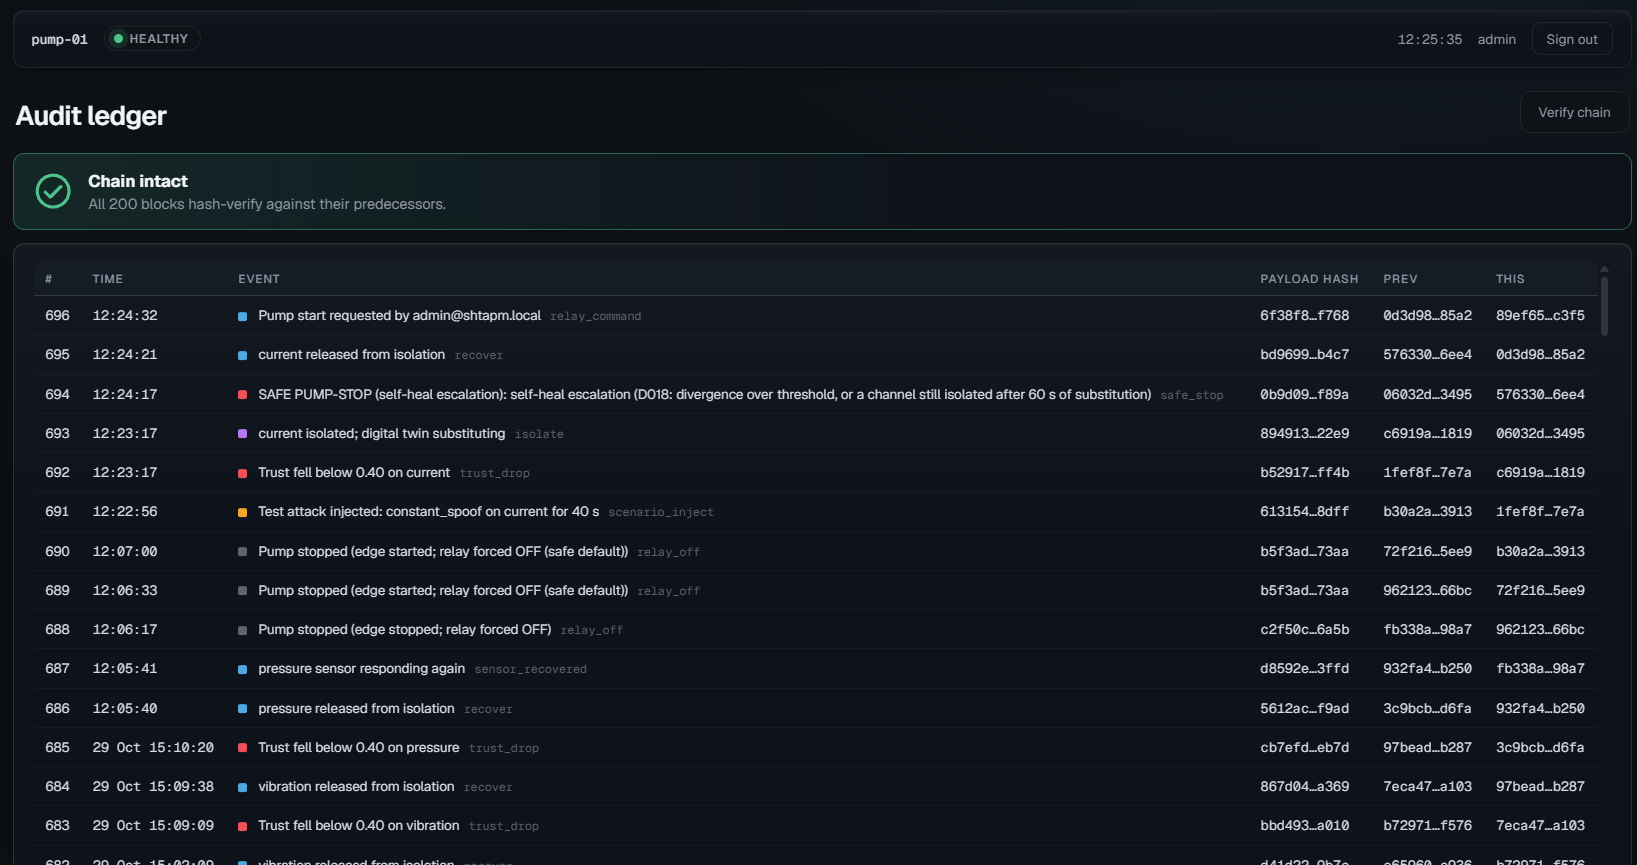
\includegraphics[width=\textwidth]{figures/ledger.png}
\caption{Audit ledger after chain verification, showing the injection, trust drop, isolation, safe stop and release of the live incident.}
\label{fig:ledger}
\end{figure}

\subsection{Alerts, Condition Rollup and Access Control}

The backend raises one alert per incident at the moments the ledger records them: a trust drop (critical, labelled attack or fault from the edge's attribution), a safe stop (critical) and a dead sensor (warning). A device-condition rollup reports \emph{critical} on a latched safe stop, attacks in a majority (5) of the last 10 decisions, or an isolated channel under a fresh attack; \emph{warning} on an isolated channel or faults and attacks in a majority of the last 10; and \emph{healthy} otherwise. It is condition monitoring, not prognosis, and it never presents a remaining-life estimate. Passwords are hashed with bcrypt; access tokens last 15 minutes and refresh tokens, valid for 7 days, are rotated on use and revoked on logout. Three roles apply: operators view and acknowledge; analysts additionally verify the ledger and inject test scenarios; administrators additionally switch the pump and manage users, devices and thresholds. A scenario injection by an operator is refused and the denial is written to the audit log.

\subsection{Dashboard Design}

The dashboard follows the principles of ANSI/ISA-101 \cite{isa101}: it is calm and neutral during normal operation, colour is reserved for abnormal states, and every state is also written in words (\textsc{attack}, \textsc{fault}, \textsc{virtual}) so that it is readable without colour. Every verdict shows its reason, and every isolation shows the twin's value next to the sensor's rejected reading so that the operator can check the system's reasoning (Figs.~\ref{fig:ui} and~\ref{fig:normal}). A fault is shown only when it holds 5 of the last 10 decisions, so a single noisy window does not alarm the operator, and a channel silent for 10~s is shown as \textsc{no data} instead of with a stale value.

\begin{figure}[H]
\centering
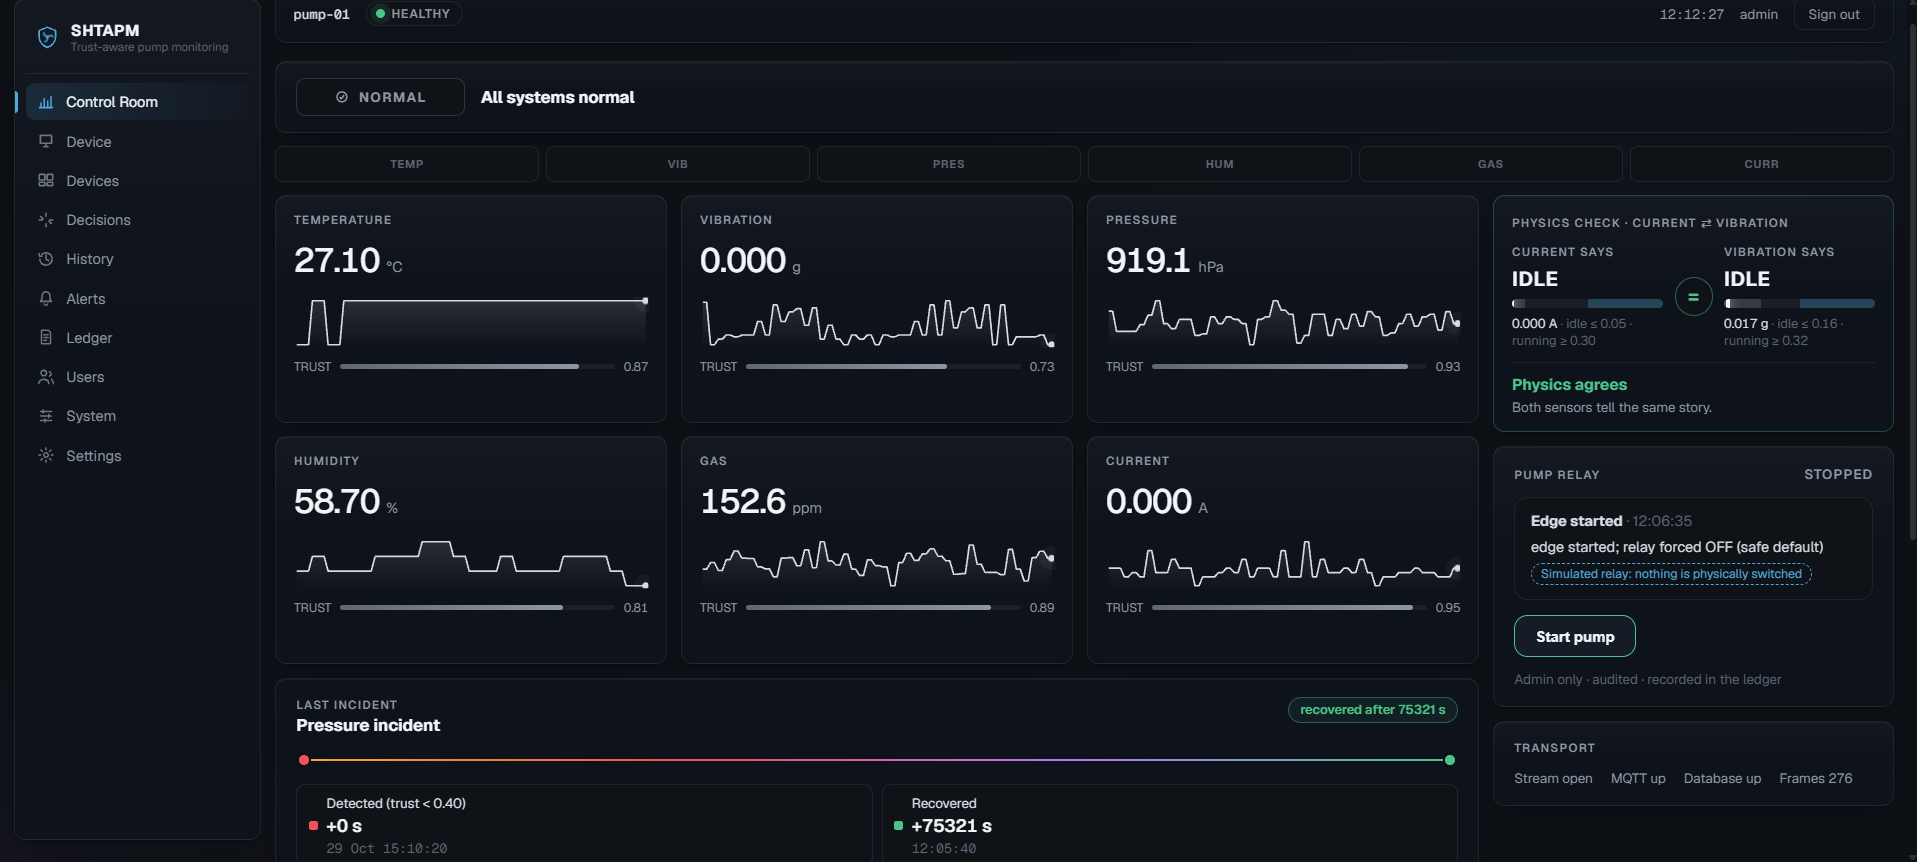
\includegraphics[width=\textwidth]{figures/controlroom-normal.png}
\caption{Control room during normal operation, with the motor idle and both physical witnesses agreeing.}
\label{fig:normal}
\end{figure}

%==============================================================
\section{Discussion and Security Considerations}
\label{sec:discussion}

\subsection{Why an Accusation Must Never Be False}

The operating-state rule trades some attack recall for an accusation that is never false on clean data. We consider this the property that matters to an operator: a false accusation triggers a security response against a healthy sensor, whereas a missed attack in a state-consistent form is exactly the case that no physical rule can see. The trend-sign baseline illustrates the failure mode of the opposite trade. Its high apparent recall comes from labelling most anomalies as attacks, which raises the false-alarm burden, and it labelled genuine physical events as attacks.

\subsection{Trust Dynamics and Hysteresis}

Two asymmetries in the design protect against both false isolation and premature release. Trust falls within three windows of adverse evidence but needs about 21 clean windows to recover, so a sensor that has lied must earn trust back; and a channel is isolated below 0.4 but released only at 0.7, so a channel whose trust wanders inside the Suspicious band neither flickers into isolation nor is released early.

\subsection{Bounded Substitution as a Safety Argument}

The twin's value is accurate for tens of seconds (Table~\ref{tab:heal}), but a reconstruction is never a measurement. The substitution budget therefore ends in a latched safe stop: a falsified sensor can cause the pump to stop, which costs availability, but cannot cause the plant to run indefinitely on a model. The same reasoning applies to the dry-run rule, which reads the current channel: spoofing current into the dry-run band forces a stop (lost availability, never lost safety), and spoofing normal current during a genuine dry run would hide it, which is a residual risk that physical redundancy on a real pump would reduce.

\subsection{Generalisation to Full-Scale Pumps}

The rule uses only the coarse fact that a running motor draws current and vibrates. On a full-scale pump, discharge pressure and flow add further physically coupled witnesses, so attacks on pressure and other channels could be attributed as well, and the vibration bands would be learned from a baseline on the actual installation by the same procedure used here.

%==============================================================
\section{Limitations}
\label{sec:limits}

\subsection{Within-State Attacks}

A falsification that keeps a reading inside its true physical state is consistent with all other sensors and cannot be attributed by the physics rule (0 of 23 in Table~\ref{tab:attr}); the twin exposes only large in-state deviations (Table~\ref{tab:residual}).

\subsection{Drift versus Ramp}

A gradual drift fault and a ramp attack have the same waveform and cannot be separated without additional evidence; most remaining fault errors are drifts.

\subsection{Coverage of Physical Coupling}

Only current and vibration have a physical partner on the bench; the other channels can be attributed only as faults.

\subsection{Prototype Scope}

A small DC motor stands in for the pump, so dry-run protection was verified on injected frames and not on a real dry run; the gas channel and the relay were exercised through emulated sources; the bench broker was unauthenticated; and remaining-useful-life prognosis and a learned response policy are implemented as modules but not deployed, because they need run-to-failure data from the target pump and agreed reward weights respectively. Validation on a full-scale pump with a physical relay and gas sensor, broker authentication with TLS, and a database migration to PostgreSQL with TimescaleDB are the natural next steps.

%==============================================================
\section{Conclusion}
\label{sec:conclusion}

This paper presented SHTAPM, a framework that keeps an industrial pump monitored and accountable while one of its sensors is failing or falsified. Physical redundancy between two inexpensive sensors, whether the motor draws current and whether it vibrates, turns ``something is anomalous'' into ``this sensor is lying'' without a dynamic process model. Combined with evidence-fusing trust whose steady state equals its evidence, bounded digital-twin substitution, a latched safe stop and a hash-chained decision ledger, the framework produced no false attack attribution on 2,552 clean channel-windows, attributed 73\% of state-crossing attacks while keeping 85\% of faults as faults, reduced the error under attack by 79--87\% out of sample, and stopped the pump exactly at its 60~s budget in a live test. The evaluation also states precisely where physical evidence runs out. Future work will validate the framework on a full-scale pump with a physical relay and gas sensor, add physically coupled channels such as discharge pressure, and combine physical attribution with sensor attestation to address within-state attacks.

\section*{Declarations}

\textbf{Funding.} No external funding was received for this work.

\textbf{Conflict of Interest.} The authors declare no conflict of interest.

\textbf{Author Contributions.} Tejashwini A G supervised the work. Durgashree R, Keerthi S and Yeshwanth L B carried out the design, implementation, experiments and writing.

\textbf{Data Availability.} The SWaT dataset is available from the iTrust Centre for Research in Cyber Security on request. The bench recordings and the source code are not public and are available from the authors on reasonable request.

%%BIB%%
\begin{thebibliography}{99}
\small
\setlength{\itemsep}{3pt}

\bibitem{ahmed2017wadi} C. M. Ahmed, V. R. Palleti, and A. P. Mathur. WADI: A water distribution testbed for research in the design of secure cyber physical systems. In Proc. 3rd International Workshop on Cyber-Physical Systems for Smart Water Networks (CySWATER), ACM, pages 25--28, 2017.

\bibitem{ahmed2018noise} C. M. Ahmed, J. Zhou, and A. P. Mathur. Noise matters: Using sensor and process noise fingerprint to detect stealthy cyber attacks and authenticate sensors in CPS. In Proc. 34th Annual Computer Security Applications Conference (ACSAC), pages 566--581, 2018.

\bibitem{almiani2020rnn} M. Almiani, A. AbuGhazleh, A. Al-Rahayfeh, S. Atiewi, and A. Razaque. Deep recurrent neural network for IoT intrusion detection system. Simulation Modelling Practice and Theory, 101(102031):102031, 2020.

\bibitem{cardenas2011attacks} A. A. C\'ardenas, S. Amin, Z.-S. Lin, Y.-L. Huang, C.-Y. Huang, and S. Sastry. Attacks against process control systems: Risk assessment, detection, and response. In Proc. 6th ACM Symposium on Information, Computer and Communications Security (ASIACCS), pages 355--366, 2011.

\bibitem{bao2012dynamic} F. Bao and I.-R. Chen. Dynamic trust management for Internet of Things applications. In Proc. International Workshop on Self-Aware Internet of Things (Self-IoT), San Jose, CA, USA, pages 1--6, 2012.

\bibitem{mitchell2014ids} R. Mitchell and I.-R. Chen. A survey of intrusion detection techniques for cyber-physical systems. ACM Computing Surveys, 46(4):55, 2014.

\bibitem{bao2012trust} F. Bao and I.-R. Chen. Trust management for the Internet of Things and its application to service composition. In Proc. IEEE International Symposium on a World of Wireless, Mobile and Multimedia Networks (WoWMoM), pages 1--6, 2012.

\bibitem{ding2018survey} D. Ding, Q.-L. Han, Y. Xiang, X. Ge, and X.-M. Zhang. A survey on security control and attack detection for industrial cyber-physical systems. Neurocomputing, 275:1674--1683, 2018.

\bibitem{dorri2017optimized} A. Dorri, S. S. Kanhere, and R. Jurdak. Towards an optimized blockchain for IoT. In Proc. IEEE/ACM Second International Conference on Internet-of-Things Design and Implementation (IoTDI), pages 173--178, 2017.

\bibitem{ganeriwal2008reputation} S. Ganeriwal, L. K. Balzano, and M. B. Srivastava. Reputation-based framework for high integrity sensor networks. ACM Transactions on Sensor Networks, 4(3):15:1--15:37, 2008.

\bibitem{giraldo2018physics} J. Giraldo, D. Urbina, A. C\'ardenas, J. Valente, M. Faisal, J. Ruths, N. O. Tippenhauer, H. Sandberg, and R. Candell. A survey of physics-based attack detection in cyber-physical systems. ACM Computing Surveys, 51(4):76:1--76:36, 2018.

\bibitem{goh2016swat} J. Goh, S. Adepu, K. N. Junejo, and A. Mathur. A dataset to support research in the design of secure water treatment systems. In Proc. International Conference on Critical Information Infrastructures Security (CRITIS), Springer LNCS 10242, pages 88--99, 2017.

\bibitem{goh2017rnn} J. Goh, S. Adepu, M. Tan, and Z. S. Lee. Anomaly detection in cyber physical systems using recurrent neural networks. In Proc. IEEE 18th International Symposium on High Assurance Systems Engineering (HASE), pages 140--145, 2017.

\bibitem{humayed2017cps} A. Humayed, J. Lin, F. Li, and B. Luo. Cyber-physical systems security---A survey. IEEE Internet of Things Journal, 4(6):1802--1831, 2017.

\bibitem{isa101} International Society of Automation. \emph{ANSI/ISA-101.01-2015: Human Machine Interfaces for Process Automation Systems}. Research Triangle Park, NC, USA, 2015.

\bibitem{isermann2005fdd} R. Isermann. Model-based fault-detection and diagnosis---Status and applications. Annual Reviews in Control, 29(1):71--85, 2005.

\bibitem{josang2002beta} A. J{\o}sang and R. Ismail. The beta reputation system. In Proc. 15th Bled Electronic Commerce Conference, pages 2502--2511, 2002.

\bibitem{kolias2017mirai} C. Kolias, G. Kambourakis, A. Stavrou, and J. Voas. DDoS in the IoT: Mirai and other botnets. Computer, 50(7):80--84, 2017.

\bibitem{langner2011stuxnet} R. Langner. Stuxnet: Dissecting a cyberwarfare weapon. IEEE Security \& Privacy, 9(3):49--51, 2011.

\bibitem{lee2014phm} J. Lee, F. Wu, W. Zhao, M. Ghaffari, L. Liao, and D. Siegel. Prognostics and health management design for rotary machinery systems---Reviews, methodology and applications. Mechanical Systems and Signal Processing, 42(1--2):314--334, 2014.

\bibitem{lee2015cps} J. Lee, B. Bagheri, and H.-A. Kao. A cyber-physical systems architecture for Industry 4.0-based manufacturing systems. Manufacturing Letters, 3:18--23, 2015.

\bibitem{liu2008iforest} F. T. Liu, K. M. Ting, and Z.-H. Zhou. Isolation forest. In Proc. 8th IEEE International Conference on Data Mining (ICDM), pages 413--422, 2008.

\bibitem{liu2009fdi} Y. Liu, P. Ning, and M. K. Reiter. False data injection attacks against state estimation in electric power grids. In Proc. 16th ACM Conference on Computer and Communications Security (CCS), pages 21--32, 2009.

\bibitem{malhotra2015lstm} P. Malhotra, L. Vig, G. Shroff, and P. Agarwal. Long short term memory networks for anomaly detection in time series. In Proc. European Symposium on Artificial Neural Networks (ESANN), pages 89--94, 2015.

\bibitem{mnih2015dqn} V. Mnih, K. Kavukcuoglu, D. Silver, A. A. Rusu, J. Veness, and M. G. Bellemare \emph{et al.}. Human-level control through deep reinforcement learning. Nature, 518(7540):529--533, 2015.

\bibitem{motmi2022elithe} A. Motmi, S. Alhazmi, A. Abu-Khadrah, M. Al-Akhras, and F. Alhosban. Trust management in Industrial Internet of Things using a trusted E-Lithe protocol. International Journal of Advanced Computer Science and Applications, 13(2), 2022.

\bibitem{nakamoto2008bitcoin} S. Nakamoto. Bitcoin: A peer-to-peer electronic cash system. 2008. Available online at bitcoin.org

\bibitem{nectoux2012pronostia} P. Nectoux, R. Gouriveau, K. Medjaher, E. Ramasso, B. Chebel-Morello, N. Zerhouni, and C. Varnier. PRONOSTIA: An experimental platform for bearings accelerated degradation tests. In Proc. IEEE International Conference on Prognostics and Health Management (PHM), Denver, CO, USA, pages 1--8, 2012.

\bibitem{pasqualetti2013identification} F. Pasqualetti, F. D\"orfler, and F. Bullo. Attack detection and identification in cyber-physical systems. IEEE Transactions on Automatic Control, 58(11):2715--2729, 2013.

\bibitem{purohit2019mimii} H. Purohit, R. Tanabe, K. Ichige, T. Endo, Y. Nikaido, K. Suefusa, and Y. Kawaguchi. MIMII dataset: Sound dataset for malfunctioning industrial machine investigation and inspection. In Proc. Detection and Classification of Acoustic Scenes and Events Workshop (DCASE), pages 209--213, 2019.

\bibitem{ran2019pdmsurvey} Y. Ran, X. Zhou, P. Lin, Y. Wen, and R. Deng. A survey of predictive maintenance: Systems, purposes and approaches. arXiv preprint arXiv:1912.07383, 2019.

\bibitem{smith2015cwru} W. A. Smith and R. B. Randall. Rolling element bearing diagnostics using the Case Western Reserve University data: A benchmark study. Mechanical Systems and Signal Processing, 64--65:100--131, 2015.

\bibitem{nguyen2023drl} T. T. Nguyen and V. J. Reddi. Deep reinforcement learning for cyber security. IEEE Transactions on Neural Networks and Learning Systems, 34(8):3779--3795, 2023.

\bibitem{roman2013features} R. Roman, J. Zhou, and J. Lopez. On the features and challenges of security and privacy in distributed Internet of Things. Computer Networks, 57(10):2266--2279, 2013.

\bibitem{saxena2008cmapss} A. Saxena, K. Goebel, D. Simon, and N. Eklund. Damage propagation modeling for aircraft engine run-to-failure simulation. In Proc. International Conference on Prognostics and Health Management (PHM), Denver, CO, USA, pages 1--9, 2008.

\bibitem{hochreiter1997lstm} S. Hochreiter and J. Schmidhuber. Long short-term memory. Neural Computation, 9(8):1735--1780, 1997.

\bibitem{kravchik2018cnn} M. Kravchik and A. Shabtai. Detecting cyber attacks in industrial control systems using convolutional neural networks. In Proc. Workshop on Cyber-Physical Systems Security and Privacy (CPS-SPC), ACM, pages 72--83, 2018.

\bibitem{sicari2015road} S. Sicari, A. Rizzardi, L. A. Grieco, and A. Coen-Porisini. Security, privacy and trust in Internet of Things: The road ahead. Computer Networks, 76:146--164, 2015.

\bibitem{mo2009replay} Y. Mo and B. Sinopoli. Secure control against replay attacks. In Proc. 47th Annual Allerton Conference on Communication, Control, and Computing, pages 911--918, 2009.

\bibitem{haber1991timestamp} S. Haber and W. S. Stornetta. How to time-stamp a digital document. Journal of Cryptology, 3(2):99--111, 1991.

\bibitem{susto2015pdm} G. A. Susto, A. Schirru, S. Pampuri, S. McLoone, and A. Beghi. Machine learning for predictive maintenance: A multiple classifier approach. IEEE Transactions on Industrial Informatics, 11(3):812--820, 2015.

\bibitem{tao2019twin} F. Tao, H. Zhang, A. Liu, and A. Y. C. Nee. Digital twin in industry: State-of-the-art. IEEE Transactions on Industrial Informatics, 15(4):2405--2415, 2019.

\bibitem{teixeira2015secure} A. Teixeira, I. Shames, H. Sandberg, and K. H. Johansson. A secure control framework for resource-limited adversaries. Automatica, 51:135--148, 2015.

\bibitem{urbina2016stealthy} D. I. Urbina, J. A. Giraldo, A. A. C\'ardenas, N. O. Tippenhauer, J. Valente, M. Faisal, J. Ruths, R. Candell, and H. Sandberg. Limiting the impact of stealthy attacks on industrial control systems. In Proc. ACM SIGSAC Conference on Computer and Communications Security (CCS), pages 1092--1105, 2016.

\bibitem{wang2023container} R. Wang, H. Qiu, X. Cheng, and X. Liu. Anomaly detection with a container-based stream processing framework for Industrial Internet of Things. Journal of Industrial Information Integration, 35, 2023.

\bibitem{chow1984redundancy} E. Y. Chow and A. S. Willsky. Analytical redundancy and the design of robust failure detection systems. IEEE Transactions on Automatic Control, 29(7):603--614, 1984.

\bibitem{yan2014trust} Z. Yan, P. Zhang, and A. V. Vasilakos. A survey on trust management for Internet of Things. Journal of Network and Computer Applications, 42:120--134, 2014.

\bibitem{zhang2017wdcnn} W. Zhang, G. Peng, C. Li, Y. Chen, and Z. Zhang. A new deep learning model for fault diagnosis with good anti-noise and domain adaptation ability on raw vibration signals. Sensors, 17(2):425, 2017.

\bibitem{zhao2019dlhealth} R. Zhao, R. Yan, Z. Chen, K. Mao, P. Wang, and R. X. Gao. Deep learning and its applications to machine health monitoring. Mechanical Systems and Signal Processing, 115:213--237, 2019.

\end{thebibliography}

\end{document}
